\section{Forward Sampling Strategies}
\label{sec:forwardSamplingStrategies}
In order to perform UQ and dynamic
probabilistic risk assessment (DPRA),
a sampling strategy needs to be employed. The sampling strategy aims to
perturb the input space (domain of the uncertainties) to explore
the response of a complex system in relation to selected FOMs.
\\The most widely used strategies to perform UQ and PRA are generally
collected into the category that, in RAVEN, is called \textit{\textbf{Forward}} samplers. The \textit{\textbf{Forward}} sampler category collects all the strategies that perform the sampling of the input space without exploiting, through learning approaches, the information made available from the outcomes of evaluation previously performed (adaptive sampling) and the common system evolution (patterns) that different sampled calculations can generate in the phase space (Dynamic Event Tree).
\\As mentioned in Section~\ref{susub:OverviewSamplers}, RAVEN has
different \textit{\textbf{Forward}} samplers:
\begin{itemize}
  \item \textit{Monte-Carlo}
  \item \textit{Grid-based}
  \item \textit{Stratified} and its specialization named \textit{Latin Hyper Cube}.
\end{itemize}
In addition, RAVEN posses advanced \textit{\textbf{Forward}} sampling strategies that:
\begin{itemize}
  \item Build a grid in the input space selecting evaluation points
  based on characteristic quadratures as part of stochastic collocation
  for generalized polynomial chaos method (\textit{Sparse
  Grid Collocation} sampler);
  \item Use high-density model reduction (HDMR) a.k.a. Sobol
  decomposition to approximate a function as the sum of increasing
  complexity interactions (\textit{Sobol} sampler).
\end{itemize}
In the following subsections, the theory behind these sampling
methodologies is going to be explained by way of applied RAVEN
examples.
%%%%%%%%%%%%%%%%%%%%%%%%%
%%%%%%%%  MONTE-CARLO %%%%%%%%
%%%%%%%%%%%%%%%%%%%%%%%%%
\subsection{Monte-Carlo}
\label{sub:MC}
The Monte-Carlo method is probably one of the most used methodologies in several disciplines. In this section, a brief theoretical
background is reported. In addition,it is shown how to employ this methodology with RAVEN.
\subsubsection{Monte-Carlo}
\label{subsub:MCtheory}
The Monte-Carlo method approximates an expectation by the sample mean of a function of
simulated random variables. It is based on the laws of large numbers in order to approximate expectations.
In order words, it approximates the average response of multiple FOMs
relying on multiple random sampling of the input space.
\\Consider a random variable (eventually multidimensional) $X$ having probability mass function or probability density function $pdf_{X}(x)$,
which is greater than zero on a set of values $\chi$. Then the expected value of a function $f$ of $X$ is as follows:
\begin{equation}
\begin{matrix}
\mathbb{E}(f(X)) =\sum_{x \in \chi} f(x)pdf_{X}(x) & \text{if} X \, discrete \\
\\
\mathbb{E}(f(X)) =\int_{x \in \chi} f(x)pdf_{X}(x) & \, \text{if} X \, \, continuous
\end{matrix}
\end{equation}
Now consider $n$ samples of $X$, $(x_{1},...,x_{n})$, and compute the mean of $f(x)$ over the samples. This computation represents the Monte-Carlo estimate:
\begin{equation}
  \mathbb{E}(f(X)) \approx   \widetilde{f}_{n}(x) = \frac{1}{n} \sum_{i=1}^{n} f(x_{i})
\end{equation}
If $\mathbb{E}(f(X))$ exists, then the law of large numbers determines that for any arbitrarily small $\varepsilon$:
\begin{equation}
  \lim_{n\rightarrow \, \infty} P( \left | \widetilde{f}_{n}(X) - \mathbb{E}(f(X))  \right |\geq \varepsilon) = 0
\end{equation}
The above equation suggests that as $n$ gets larger, then the probability that $\widetilde{f}_{n}(X)$ deviates
from the $\mathbb{E}(f(X))$ becomes smaller. In other words, the more samples are spooned, the more closer the Monte-Carlo estimate of $X$ gets to the real value.
\\In addition, $\widetilde{f}_{n}(X)$ represent an unbiased estimate for $\mathbb{E}(f(X))$:
\begin{equation}
\mathbb{E}(\widetilde{f}_{n}(X)) = \mathbb{E} \left ( \frac{1}{n} \sum_{i=1}^{n} f(x_{i})   \right ) =
\frac{1}{n} \sum_{i=1}^{n} \mathbb{E}(f(x_{i})) =   \mathbb{E}(f(X))
\end{equation}
%After this brief introduction, it is important to understand how the Monte-Carlo method can be employed
%for the analysis of Dynamic Stochastic system.
%\\Referencing to the nomenclature defined in section~\ref{sub:mathBackground}, given:
%\begin{equation}
%\frac{\partial  \overline{\theta}^{c}\left ( t \right )}{\partial t}=f\left ( \overline{\theta}^{c},\overline{\theta}^{d}_{i}, \overline{\alpha}_{staz} ,\overline{\alpha}_{brow}, t \right )
%\end{equation}
% define a function $g_{i}$ that represents the solution of the previous equation (the trajectory in the $ \overline{\theta}^{c}$ space for a fixed $ \overline{\theta}^{d}_{i}$ and initial condition $\overline{\theta}^{c}_{0}$) :
%\begin{equation}
%  \overline{\theta}^{c}(t) = g_{i}(t,\overline{\theta}^{c}_{0})
%\end{equation}
%The Monte-Carlo analysis is performed as following:
%\begin{enumerate}
%  \item Sample:
%  \begin{itemize}
%    \item $\overline{\alpha}_{staz} $,$\overline{\alpha}_{DS}$, $\overline{t}$ depending on which
%    approximations are valid (see~\ref{sub:mathBackground});
%    \item The initial conditions $\overline{\theta}^{c}_{0}$,$\overline{\theta}^{d}_{0}$;
%    \item Transition conditions from $W(\overline{\theta}^{d}|\overline{\theta}^{d}_{i},\overline{\theta}^{c},t)$
%  \end{itemize}
%  \item Run the system simulator using the previously sampled values and affected by the intrinsic stochasticity
%  represented by $\overline{\alpha}_{brow}$;
%  \item Pause the simulation when a transition condition is reached and move from the current $\overline{\theta}^{d}_{0}$ to the new $\overline{\theta}^{d}$ (e.g. $\overline{\theta}^{d}_{1}$);
%  \item Run the simulation as performed in step 3, starting from the new coordinate and pause the simulation when a new transition is reached;
%  \item Repeat steps 3 and 4 until a stopping condition is reached;
%  \item Repeat 1 through 4 for a large number of runs $n$.
%\end{enumerate}
\subsubsection{Monte-Carlo sampling through RAVEN}
\label{subsub:MCexample}
The goals of this section are about learning how to:
 \begin{enumerate}
   \item Set up a simple Monte-Carlo sampling for perturbing the input
   space of a driven code
   \item Load the outputs of the code into the RAVEN DataObjects
   system (HistorySet and PointSet)
   \item Print on file what contained in the DataObjects
   \item Generate plots of the code results.
\end{enumerate}
In order to accomplish these tasks, the following RAVEN \textbf{Entities} (XML blocks in the input files) are needed:
\begin{enumerate}
   \item \textbf{\textit{RunInfo}}:
\begin{lstlisting}[style=XML,morekeywords={arg,extension,pauseAtEnd,overwrite}]
  <RunInfo>
    <JobName>ChapterVII-I/MonteCarlo</JobName>
    <Sequence>sample,writeHistories</Sequence>
    <WorkingDir>ChapterVII-I/MonteCarlo</WorkingDir>
    <batchSize>12</batchSize>
  </RunInfo>
\end{lstlisting}
   As reported in Section~\ref{sub:EntitiesAndFlow}, the \textit{RunInfo} \textbf{Entity} is intended to set up the analysis
   that the user wants to perform. In this specific case, two steps (\xmlNode{Sequence}) are sequentially run
   using 12 processors (\xmlNode{batchSize}). This means that
   12 instances of the driven code are run simultaneously.
   Every time a simulation ends, a new one is launched.
   \item \textbf{\textit{Files}}:
\begin{lstlisting}[style=XML,morekeywords={arg,extension,pauseAtEnd,overwrite}]
  <Files>
    <Input name="referenceInput.xml" type="input">referenceInput.xml</Input>
  </Files>
\end{lstlisting}
   Since the driven code uses a single input file, in this section the original input is placed. As detailed in the user manual
   the attribute  \xmlAttr{name} represents the alias that is going to be used in all the other input blocks in order to refer to this file.
   \item \textbf{\textit{Models}}:
\begin{lstlisting}[style=XML,morekeywords={arg,extension,pauseAtEnd,overwrite}]
   <Models>
      <Code name="testModel" subType="GenericCode">
        <executable>
    ../physicalCode/analyticalbateman/AnalyticalDplMain.py
        </executable>
        <clargs arg="python" type="prepend"/>
        <clargs arg="" extension=".xml" type="input"/>
        <clargs arg="" extension=".csv" type="output"/>
        <prepend>python</prepend>
      </Code>
    <Models>
\end{lstlisting}
 The Model here is represented by the
 \textbf{AnalyticalBateman}, which already exports its output file in a
 CSV format (standard format that RAVEN can read). For this reason,
 the \textit{GenericCode} interface is used.
   \item \textbf{\textit{Distributions}}:
\begin{lstlisting}[style=XML,morekeywords={arg,extension,pauseAtEnd,overwrite}]
  <Distributions>
      <Uniform name="sigma">
          <lowerBound>1</lowerBound>
          <upperBound>10</upperBound>
      </Uniform>
      <Uniform name="decayConstant">
          <lowerBound>0.000000005</lowerBound>
          <upperBound>0.000000010</upperBound>
      </Uniform>
  </Distributions>
\end{lstlisting}
  In the Distributions XML section, the stochastic model for the
  uncertainties  treated by the Monte-Carlo sampling is reported. In
  this case two distributions are defined:
  \begin{itemize}
    \item $sigma \sim \mathbb{U}(1,10)$, used to model the uncertainties
    associated with  the Model \textit{sigma}(s)
    \item  $decayConstant \sim \mathbb{U}(0.5e-8,1e-8)$,  used to
    model the uncertainties
    associated with  the Model \textit{decay constants}.
  \end{itemize}
   \item \textbf{\textit{Samplers}}:
\begin{lstlisting}[style=XML,morekeywords={arg,extension,pauseAtEnd,overwrite}]
  <Samplers>
    <MonteCarlo name="monteCarlo">
        <samplerInit>
            <limit>100</limit>
        </samplerInit>
      <variable name="sigma-A">
        <distribution>sigma</distribution>
      </variable>
      <variable name="decay-A">
        <distribution>decayConstant</distribution>
      </variable>
      <variable name="sigma-B">
          <distribution>sigma</distribution>
      </variable>
      <variable name="decay-B">
          <distribution>decayConstant</distribution>
      </variable>
      <variable name="sigma-C">
          <distribution>sigma</distribution>
      </variable>
      <variable name="decay-C">
          <distribution>decayConstant</distribution>
      </variable>
      <variable name="sigma-D">
          <distribution>sigma</distribution>
      </variable>
      <variable name="decay-D">
          <distribution>decayConstant</distribution>
      </variable>
    </MonteCarlo>
  </Samplers>
\end{lstlisting}
  To employ the Monte-Carlo sampling strategy ($100$ samples), a
  \xmlNode{MonteCarlo} node needs to be inputted.  The
  Monte-Carlo method is going to be employed on $eight$ model variables.
  Note that all the \textit{decay-\%} and
  \textit{sigma-\%} variables are associated with the same distributions
  $decayConstant$ and $sigma$, respectively.
   \item \textbf{\textit{DataObjects}}:
\begin{lstlisting}[style=XML,morekeywords={arg,extension,pauseAtEnd,overwrite}]
  <DataObjects>
    <PointSet name="samples">
      <Input>
        sigma-A,sigma-B,sigma-C,sigma-D,
        decay-A,decay-B,decay-C,decay-D
      </Input>
      <Output>A,B,C,D,time</Output>
    </PointSet>
    <HistorySet name="histories">
        <Input>
          sigma-A,sigma-B,sigma-C,sigma-D,
          decay-A,decay-B,decay-C,decay-D
        </Input>
        <Output>A,B,C,D,time</Output>
    </HistorySet>
  </DataObjects>
\end{lstlisting}
  Int this block, two \textit{DataObjects} are defined: 1) PointSet named
  ``samples'', 2) HistorySet named ``histories''.
  Note that in the \xmlNode{Input} node all the uncertainties
  perturbed through the Monte-Carlo strategy are listed. By this, any
  realization in the input space is linked to the outputs listed in the
  \xmlNode{Output} node.
   \item \textbf{\textit{OutStreams}}:
\begin{lstlisting}[style=XML,morekeywords={arg,extension,pauseAtEnd,overwrite}]
  <OutStreams>
    <Print name="samples">
      <type>csv</type>
      <source>samples</source>
    </Print>
    <Print name="histories">
      <type>csv</type>
      <source>histories</source>
    </Print>
    <Plot dim="2" name="historiesPlot" overwrite="false" verbosity="debug">
        <plotSettings>
            <gridSpace>2 2</gridSpace>
            <plot>
                <type>line</type>
                <x>histories|Output|time</x>
                <y>histories|Output|A</y>
                <color>blue</color>
                <gridLocation>
                  <x>0</x>
                  <y>0</y>
                </gridLocation>
                <xlabel>time (s)</xlabel>
                <ylabel>evolution A(kg)</ylabel>
            </plot>
            <plot>
                <type>line</type>
                <x>histories|Output|time</x>
                <y>histories|Output|B</y>
                <color>red</color>
                <gridLocation>
                    <x>1</x>
                    <y>0</y>
                </gridLocation>
                <xlabel>time (s)</xlabel>
                <ylabel>evolution B(kg)</ylabel>
            </plot>
            <plot>
                <type>line</type>
                <x>histories|Output|time</x>
                <y>histories|Output|C</y>
                <color>yellow</color>
                <gridLocation>
                    <x>0</x>
                    <y>1</y>
                </gridLocation>
                <xlabel>time (s)</xlabel>
                <ylabel>evolution C(kg)</ylabel>
            </plot>
            <plot>
                <type>line</type>
                <x>histories|Output|time</x>
                <y>histories|Output|D</y>
                <color>black</color>
                <gridLocation>
                    <x>1</x>
                    <y>1</y>
                </gridLocation>
                <xlabel>time (s)</xlabel>
                <ylabel>evolution D(kg)</ylabel>
            </plot>
        </plotSettings>
        <actions>
            <how>png,screen</how>
            <title>
                <text> </text>
            </title>
        </actions>
    </Plot>
    <Plot dim="3" name="samplesPlot3D" overwrite="false" verbosity="debug">
        <plotSettings>
            <gridSpace>2 2</gridSpace>
            <plot>
                <type>scatter</type>
                <x>samples|Input|sigma-A</x>
                <y>samples|Input|decay-A</y>
                <z>samples|Output|A</z>
                <color>blue</color>
                <gridLocation>
                  <x>0</x>
                  <y>0</y>
                </gridLocation>
                <xlabel>sigma</xlabel>
                <ylabel>decay</ylabel>
                <zlabel>final A</zlabel>
            </plot>
            <plot>
                <type>scatter</type>
                <x>samples|Input|sigma-B</x>
                <y>samples|Input|decay-B</y>
                <z>samples|Output|B</z>
                <color>red</color>
                <gridLocation>
                    <x>1</x>
                    <y>0</y>
                </gridLocation>
                <xlabel>sigma</xlabel>
                <ylabel>decay</ylabel>
                <zlabel>final B</zlabel>
            </plot>
            <plot>
                <type>scatter</type>
                <x>samples|Input|sigma-C</x>
                <y>samples|Input|decay-C</y>
                <z>samples|Output|C</z>
                <color>yellow</color>
                <gridLocation>
                    <x>0</x>
                    <y>1</y>
                </gridLocation>
                <xlabel>sigma</xlabel>
                <ylabel>decay</ylabel>
                <zlabel>final C</zlabel>
            </plot>
            <plot>
                <type>scatter</type>
                <x>samples|Input|sigma-D</x>
                <y>samples|Input|decay-D</y>
                <z>samples|Output|D</z>
                <color>black</color>
                <gridLocation>
                    <x>1</x>
                    <y>1</y>
                </gridLocation>
                <xlabel>sigma</xlabel>
                <ylabel>decay</ylabel>
                <zlabel>final D</zlabel>
            </plot>
            <xlabel>sigma</xlabel>
            <ylabel>decay</ylabel>
            <zlabel>final response</zlabel>
        </plotSettings>
        <actions>
            <how>png,screen</how>
            <title>
                <text> </text>
            </title>
        </actions>
    </Plot>
  </OutStreams>
\end{lstlisting}
 %%%%%%%%%%%%%%%%%%%%%%%%%%%%%%%%%%%%%%%%%%%%%%%%%%%%%%%%%%
 %figure histories
 \begin{figure}[h!]
  \centering
  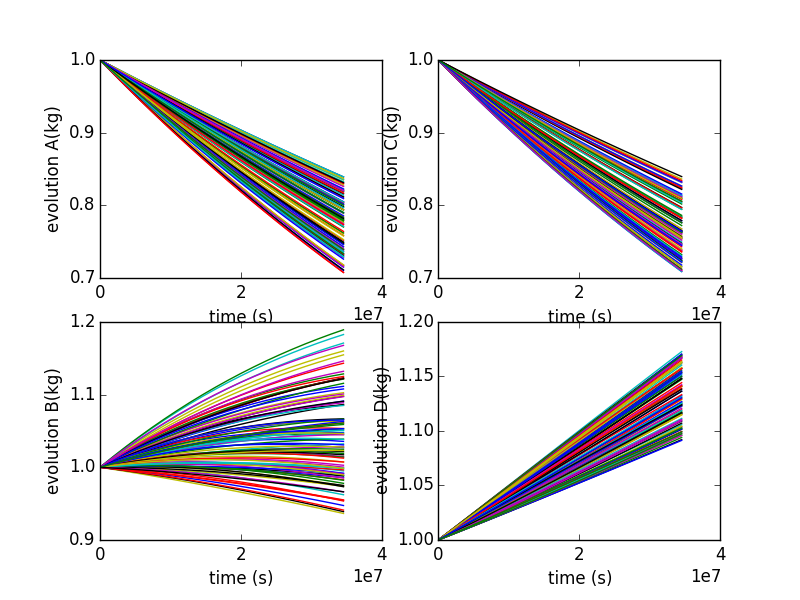
\includegraphics[scale=0.7]{pics/MC_histories.png}
  \caption{Plot of the histories generated by the Monte Carlo sampling for variables $A,B,C,D$.}
  \label{fig:historiesMCPlotLine}
 \end{figure}
 %%%%%%%%%%%%%%%%%%%%%%%%%%%%%%%%%%%%%%%%%%%%%%%%%%%%%%%%%%
  In this block, both the Out-Stream types are constructed:
  \begin{itemize}
    \item \textit{Print}:
     \begin{itemize}
       \item named ``samples'' connected with the \textit{DataObjects} \textbf{Entity} ``samples''
                (\xmlNode{source})
       \item named ``histories'' connected with the \textit{DataObjects} \textbf{Entity} ``histories'' (\xmlNode{source})
     \end{itemize}
      When these objects get used, all the information contained in the
      linked  \textit{DataObjects} are going
    to be exported in CSV files (\xmlNode{type}).
    \item \textit{Plot}:
    \begin{itemize}
      \item named ``historiesPlot'' connected with the  \textit{DataObjects}
      \textbf{Entity} ``samples''.  This plot will draw the final state of the
      variables $A,B,C,D$ with respect to the input variables $sigma$(s)
      and $decay$(s) .
      \item named ``samplesPlot3D'' connected with the
      \textit{DataObjects} \textbf{Entity} ``histories''. This plot will draw the
      evolution of the variables $A,B,C,D$;
    \end{itemize}
     Note that both plots are of type \textit{SubPlot}. Four plots
     are going to be placed in each of the figures.
  \end{itemize}
   \item \textbf{\textit{Steps}}:
\begin{lstlisting}[style=XML,morekeywords={arg,extension,pauseAtEnd,overwrite}]
  <Steps>
    <MultiRun name="sample">
      <Input 	    class="Files" 			 type="input">referenceInput.xml</Input>
      <Model 	    class="Models" 		 type="Code">testModel</Model>
      <Sampler 	class="Samplers" 		 type="MonteCarlo">monteCarlo</Sampler>
      <Output 	class="DataObjects"  type="PointSet">samples</Output>
      <Output 	class="DataObjects"  type="HistorySet">histories</Output>
    </MultiRun>
    <IOStep name="writeHistories" pauseAtEnd="True">
        <Input class="DataObjects" type="HistorySet">histories</Input>
        <Input class="DataObjects" type="PointSet">samples</Input>
        <Output 	class="OutStreams" type="Plot">samplesPlot3D</Output>
        <Output 	class="OutStreams" type="Plot">historyPlot</Output>
        <Output 	class="OutStreams" type="Print">samples</Output>
        <Output 	class="OutStreams" type="Print">histories</Output>
    </IOStep>
  </Steps>
\end{lstlisting}
 %%%%%%%%%%%%%%%%%%%%%%%%%%%%%%%%%%%%%%%%%%%%%%%%%%%%%%%%%%
 %figure samples
 \begin{figure}[h!]
  \centering
  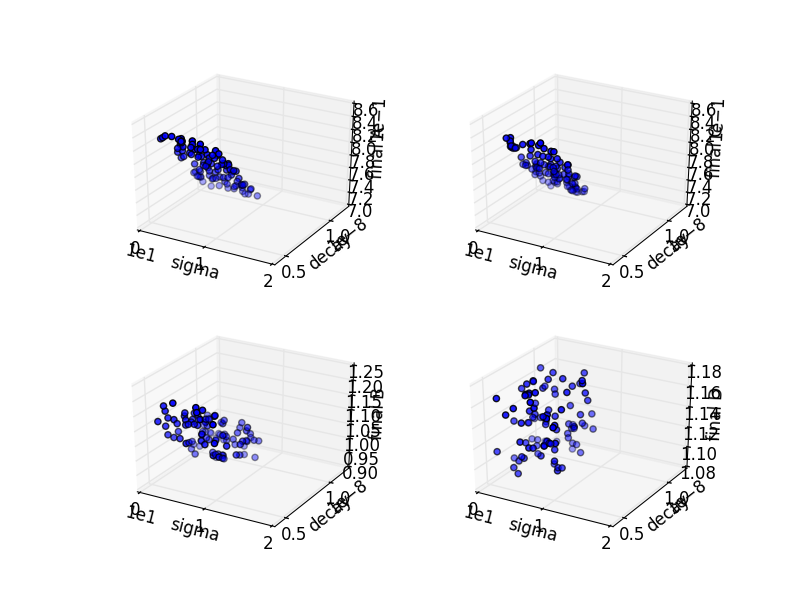
\includegraphics[scale=0.7]{pics/MC_pointsets.png}
  \caption{Plot of the samples generated by the MC sampling for variables $A,B,C,D$.}
  \label{fig:samplesMCPlotLine}
 \end{figure}
 %%%%%%%%%%%%%%%%%%%%%%%%%%%%%%%%%%%%%%%%%%%%%%%%%%%%%%%%%%
   Finally, all the previously defined \textbf{Entities} can be combined in
   the \xmlNode{Steps} block. As inferable,
   two \xmlNode{Steps} have been inputted:
   \begin{itemize}
     \item \xmlNode{MultiRun} named ``sample'', used to run the multiple
     instances of the driven code and
     collect the outputs in the two \textit{DataObjects}. As it can be
     seen, the \xmlNode{Sampler} is inputted to communicate to the
     \textit{Step} that the driven code needs to
     be perturbed through the Monte-Carlo sampling;
     \item  \xmlNode{IOStep} named ``writeHistories'', used to 1) dump
     the ``histories'' and ``samples'' \textit{DataObjects}
     \textbf{Entity} in a CSV file and 2) plot the data in the PNG file and
     on the screen.
   \end{itemize}
\end{enumerate}
 Figures~\ref{fig:historiesMCPlotLine} and ~\ref{fig:samplesMCPlotLine}  report the evolution of the
 variables $A,B,C,D$ and their final values, respectively.
%%%%%%%%%%%%%%%%%%%%%%%%%
%%%%%%%%          GRID          %%%%%%%%
%%%%%%%%%%%%%%%%%%%%%%%%%
\subsection{Grid}
\label{sub:Grid}
The Grid sampling method (also known as Full Factorial Design of Experiment) represents one of the simplest methodologies that can be employed in order to explore the interaction of multiple random variables with respect
selected FOMs.
In this section, a brief theoretical
background is reported. In addition,it is shown how to employ this methodology with RAVEN.
\subsubsection{Grid theory introduction}
\label{subsub:Gridtheory}
The goal of the Grid-based sampling strategy is to explore the interaction of multiple random
variables (i.e.,uncertainties) with respect to selected FOMs. Indeed, this method is mainly used to perform
parametric analysis of the system response rather than a probabilistic one. This method discretizes the
domain of the uncertainties in a user-defined number of intervals (see Figure~\ref{fig:GridDiscretization}) and
record the response of the model (e.g. a system code) at each coordinate (i.e., combination of the uncertainties) of the grid.
\\ This method starts from the assumption that each coordinate on the grid is representative, with respect to the FOMs of interest, of the surrounding grid cell. In other words, it is assumed that the response of a system does not significantly change within the hyper-volume surrounding each grid coordinate (red square in Figure~\ref{fig:GridDiscretization}).
 %%%%%%%%%%%%%%%%%%%%%%%%%%%%%%%%%%%%%%%%%%%%%%%%%%%%%%%%%%
 %figure history
 \begin{figure}[h!]
  \centering
  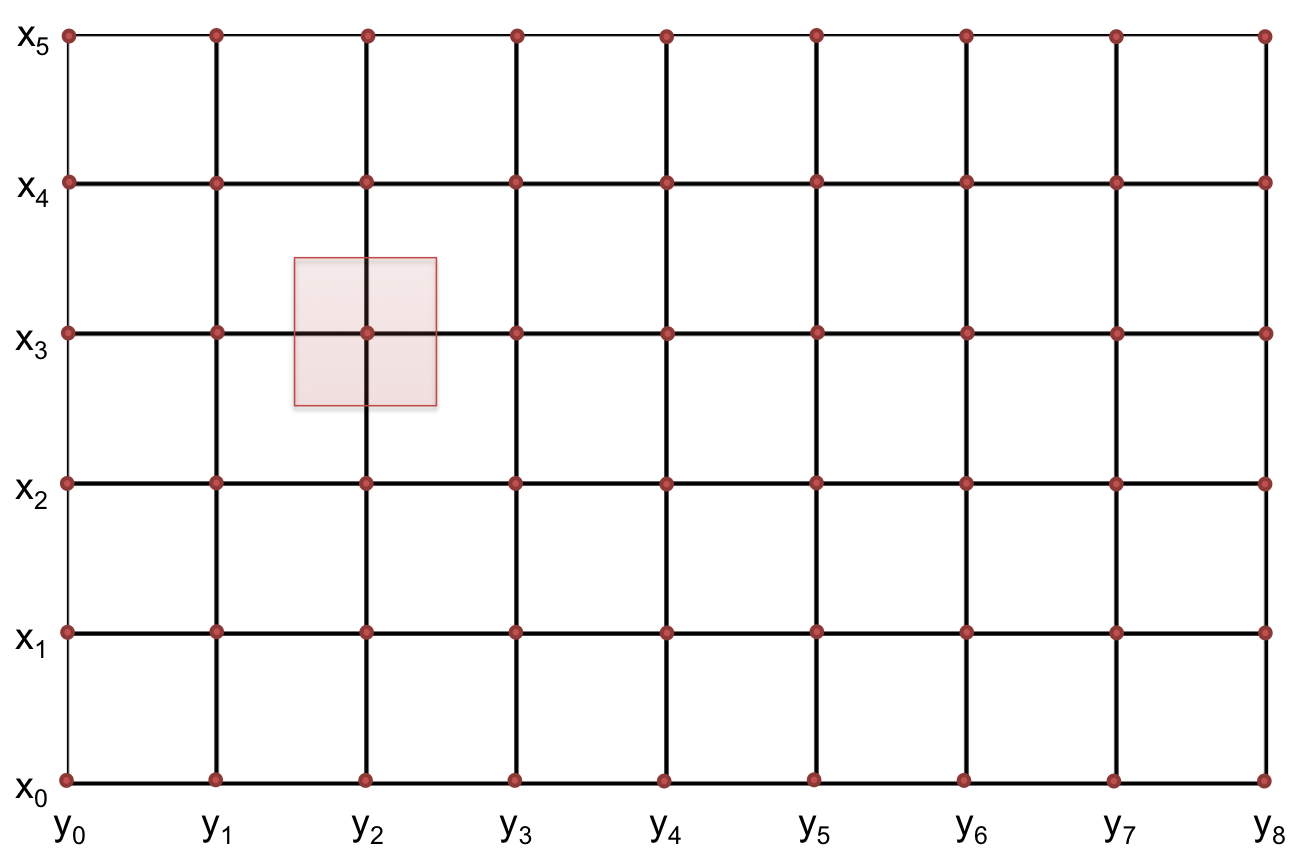
\includegraphics[scale=0.7]{pics/GridDiscretization.png}
  \caption{Example of 2-Dimensional grid discretization. }
  \label{fig:GridDiscretization}
 \end{figure}
 %%%%%%%%%%%%%%%%%%%%%%%%%%%%%%%%%%%%%%%%%%%%%%%%%%%%%%%%%%

Similarly to what has been already reported for the Monte-Carlo sampling, consider a random variable $X$ having PDF $pdf_{X}(x)$ and, consequentially, CDF $cdf_{X}(x)$ in the domain $\chi$. Then the expected value of a function $f$ of $X$ is as follows:
\begin{equation}
\begin{matrix}
\mathbb{E}(f(X)) =\sum_{x \in \chi} f(x)pdf_{X}(x) & if X \, discrete \\
\\
\mathbb{E}(f(X)) =\int_{x \in \chi} f(x)pdf_{X}(x) & \, if X \, \, continuous
\end{matrix}
\end{equation}
In the Grid approach, the domain of $X$ is discretized in a finite number of intervals. Recall that
each node of this discretization is representative of the surrounding hyper-volume. This means that a weight
needs to be associated with each coordinate of the resulting grid:
\begin{equation}
\begin{matrix}
  w_{i}= cdf_{X}(x_{i+1/2}) - cdf_{X}(x_{i-1/2})
\end{matrix}
\end{equation}
Now consider
a $n-$discretization of the domain of  $X$, $(x_{1},...,x_{n})$ and compute the mean of $f(x)$ over the discretization. Based on the previous equation, the computation of the expected value of $f(x)$ is as follows:
\begin{equation}
 \mathbb{E}(f(X)) \approx   \widetilde{f}_{n}(x) = \frac{1}{\sum_{i=1}^{n}w_{i}} \sum_{i=1}^{n} f(x_{i}) \times w_{i}
\end{equation}
If the number of uncertainties under consideration is greater than one ($m$), the above equation
becomes:
\begin{equation}
\mathbb{E}(f(\overline{X})) \approx   \widetilde{f}_{n}(\overline{x}) = \frac{1}{\sum_{i=1}^{n}\prod_{j=1}^{m}w_{i,j}} \sum_{i=1}^{n} f(\overline{x}_{i}) \times \prod_{j=1}^{m}w_{i,j}
\end{equation}

\subsubsection{Grid sampling through RAVEN}
\label{subsub:Gridexample}
The goal of this section is to show how to:
 \begin{enumerate}
   \item Set up a simple Grid sampling for performing a parametric analysis of a driven code
   \item Load the outputs of the code into the RAVEN DataObjects system
   \item Print out what contained in the DataObjects
   \item Generate basic plots of the code result.
\end{enumerate}
In order to accomplish these tasks, the following RAVEN \textbf{Entities} (XML blocks in the input files) are required:
\begin{enumerate}
   \item \textbf{\textit{RunInfo}}:
\begin{lstlisting}[style=XML,morekeywords={arg,extension,pauseAtEnd,overwrite}]
  <RunInfo>
    <JobName>ChapterVII-I/Grid</JobName>
    <Sequence>sample,writeHistories</Sequence>
    <WorkingDir>ChapterVII-I/Grid</WorkingDir>
    <batchSize>12</batchSize>
  </RunInfo>
\end{lstlisting}
   As shown in Section~\ref{sub:EntitiesAndFlow}, the \textit{RunInfo} \textbf{Entity} is intended to set up the desired analysis.
   In this specific case, two steps (\xmlNode{Sequence}) are sequentially run
   using 12 processors (\xmlNode{batchSize}). This means that
   12 instances of the driven code are  run simultaneously.
   Every time a simulation ends, a new one is launched.
   \item \textbf{\textit{Files}}:
\begin{lstlisting}[style=XML,morekeywords={arg,extension,pauseAtEnd,overwrite}]
  <Files>
    <Input name="referenceInput.xml" type="input">referenceInput.xml</Input>
  </Files>
\end{lstlisting}
   Since the driven code uses a single input file, in this section the original input is placed. As described in the user manual~\cite{RAVENuserManual}
   the attribute  \xmlAttr{name} represents the alias that is used in all the other input blocks in order to refer to this file.
   \item \textbf{\textit{Models}}:
\begin{lstlisting}[style=XML,morekeywords={arg,extension,pauseAtEnd,overwrite}]
   <Models>
      <Code name="testModel" subType="GenericCode">
        <executable>
    ../physicalCode/analyticalbateman/AnalyticalDplMain.py
        </executable>
        <clargs arg="python" type="prepend"/>
        <clargs arg="" extension=".xml" type="input"/>
        <clargs arg="" extension=".csv" type="output"/>
        <prepend>python</prepend>
      </Code>
    <Models>
\end{lstlisting}
 The Model here is represented by the
 \textbf{AnalyticalBateman}, which already dumps its output file in a
 CSV format (standard format that RAVEN can read). For this reason,
 the \textit{GenericCode} interface is used.
   \item \textbf{\textit{Distributions}}:
\begin{lstlisting}[style=XML,morekeywords={arg,extension,pauseAtEnd,overwrite}]
  <Distributions>
      <Uniform name="sigma">
          <lowerBound>1</lowerBound>
          <upperBound>10</upperBound>
      </Uniform>
      <Uniform name="decayConstant">
          <lowerBound>0.000000005</lowerBound>
          <upperBound>0.000000010</upperBound>
      </Uniform>
  </Distributions>
\end{lstlisting}
  In the Distributions XML section, the stochastic model for the
  uncertainties  treated by the Grid sampling are reported. In
  this case two distributions are defined:
  \begin{itemize}
    \item $sigma \sim \mathbb{U}(1,10)$, used to model the uncertainties
    associated with  the Model \textit{sigma}(s)
    \item  $decayConstant \sim \mathbb{U}(0.5e-8,1e-8)$,  used to
    model the uncertainties
    associated with  the Model \textit{decay constants}.
  \end{itemize}
   \item \textbf{\textit{Samplers}}:
\begin{lstlisting}[style=XML,morekeywords={arg,extension,pauseAtEnd,overwrite}]
  <Samplers>
    <Grid name="grid">
      <variable name="sigma-A">
        <distribution>sigma</distribution>
        <grid construction="equal" steps="1" type="value">2 4.0</grid>
      </variable>
      <variable name="decay-A">
        <distribution>decayConstant</distribution>
        <grid construction="custom" type="value">0.000000005  0.000000008</grid>
      </variable>
      <variable name="sigma-B">
          <distribution>sigma</distribution>
          <grid construction="equal" steps="1" type="CDF">0.1 0.8</grid>
      </variable>
      <variable name="decay-B">
          <distribution>decayConstant</distribution>
          <grid construction="equal" steps="1" type="CDF">0.1 0.8</grid>
      </variable>
      <variable name="sigma-C">
          <distribution>sigma</distribution>
          <grid construction="equal" steps="1" type="value">4 5</grid>
      </variable>
      <variable name="decay-C">
          <distribution>decayConstant</distribution>
          <grid construction="equal" steps="1" type="CDF">0.1 0.5</grid>
      </variable>
      <variable name="sigma-D">
          <distribution>sigma</distribution>
          <grid construction="equal" steps="1" type="CDF">0.4 0.8</grid>
      </variable>
      <variable name="decay-D">
          <distribution>decayConstant</distribution>
          <grid construction="equal" steps="1" type="CDF">0.1 0.8</grid>
      </variable>
    </Grid>
  </Samplers>
\end{lstlisting}
  To employ the Grid sampling strategy, a
  \xmlNode{Grid} node needs to be specified. As shown above, in each variable section, the  \xmlNode{grid} is defined.
  The number of samples finally requested are equal to $n_{samples} = \prod_{i=1}^{n} n_{steps_{i}+1} = 256$.
  Note that, for each variable, can be defined either in probability (CDF) or in absolute value.
   \item \textbf{\textit{DataObjects}}:
\begin{lstlisting}[style=XML,morekeywords={arg,extension,pauseAtEnd,overwrite}]
  <DataObjects>
    <PointSet name="samples">
      <Input>
        sigma-A,sigma-B,sigma-C,sigma-D,
        decay-A,decay-B,decay-C,decay-D
      </Input>
      <Output>A,B,C,D,time</Output>
    </PointSet>
    <HistorySet name="histories">
        <Input>
          sigma-A,sigma-B,sigma-C,sigma-D,
          decay-A,decay-B,decay-C,decay-D
        </Input>
        <Output>A,B,C,D,time</Output>
    </HistorySet>
  </DataObjects>
\end{lstlisting}
  Int this block, two \textit{DataObjects} are defined: 1) PointSet named
  ``samples'', and 2) HistorySet named ``histories''.
  In the \xmlNode{Input} node all the variables
  perturbed through the Grid strategy are listed. In this way, any
  realization in the input space is linked to the outputs listed in  the
  \xmlNode{Output} node.
   \item \textbf{\textit{OutStreams}}:
\begin{lstlisting}[style=XML,morekeywords={arg,extension,pauseAtEnd,overwrite}]
  <OutStreams>
    <Print name="samples">
      <type>csv</type>
      <source>samples</source>
    </Print>
    <Print name="histories">
      <type>csv</type>
      <source>histories</source>
    </Print>
    <Plot dim="2" name="historiesPlot" overwrite="false" verbosity="debug">
        <plotSettings>
            <gridSpace>2 2</gridSpace>
            <plot>
                <type>line</type>
                <x>histories|Output|time</x>
                <y>histories|Output|A</y>
                <color>blue</color>
                <gridLocation>
                  <x>0</x>
                  <y>0</y>
                </gridLocation>
                <xlabel>time (s)</xlabel>
                <ylabel>evolution A(kg)</ylabel>
            </plot>
            <plot>
                <type>line</type>
                <x>histories|Output|time</x>
                <y>histories|Output|B</y>
                <color>red</color>
                <gridLocation>
                    <x>1</x>
                    <y>0</y>
                </gridLocation>
                <xlabel>time (s)</xlabel>
                <ylabel>evolution B(kg)</ylabel>
            </plot>
            <plot>
                <type>line</type>
                <x>histories|Output|time</x>
                <y>histories|Output|C</y>
                <color>yellow</color>
                <gridLocation>
                    <x>0</x>
                    <y>1</y>
                </gridLocation>
                <xlabel>time (s)</xlabel>
                <ylabel>evolution C(kg)</ylabel>
            </plot>
            <plot>
                <type>line</type>
                <x>histories|Output|time</x>
                <y>histories|Output|D</y>
                <color>black</color>
                <gridLocation>
                    <x>1</x>
                    <y>1</y>
                </gridLocation>
                <xlabel>time (s)</xlabel>
                <ylabel>evolution D(kg)</ylabel>
            </plot>
        </plotSettings>
        <actions>
            <how>png,screen</how>
            <title>
                <text> </text>
            </title>
        </actions>
    </Plot>
    <Plot dim="3" name="samplesPlot3D" overwrite="false" verbosity="debug">
        <plotSettings>
            <gridSpace>2 2</gridSpace>
            <plot>
                <type>scatter</type>
                <x>samples|Input|sigma-A</x>
                <y>samples|Input|decay-A</y>
                <z>samples|Output|A</z>
                <color>blue</color>
                <gridLocation>
                  <x>0</x>
                  <y>0</y>
                </gridLocation>
                <xlabel>sigma</xlabel>
                <ylabel>decay</ylabel>
                <zlabel>final A</zlabel>
            </plot>
            <plot>
                <type>scatter</type>
                <x>samples|Input|sigma-B</x>
                <y>samples|Input|decay-B</y>
                <z>samples|Output|B</z>
                <color>red</color>
                <gridLocation>
                    <x>1</x>
                    <y>0</y>
                </gridLocation>
                <xlabel>sigma</xlabel>
                <ylabel>decay</ylabel>
                <zlabel>final B</zlabel>
            </plot>
            <plot>
                <type>scatter</type>
                <x>samples|Input|sigma-C</x>
                <y>samples|Input|decay-C</y>
                <z>samples|Output|C</z>
                <color>yellow</color>
                <gridLocation>
                    <x>0</x>
                    <y>1</y>
                </gridLocation>
                <xlabel>sigma</xlabel>
                <ylabel>decay</ylabel>
                <zlabel>final C</zlabel>
            </plot>
            <plot>
                <type>scatter</type>
                <x>samples|Input|sigma-D</x>
                <y>samples|Input|decay-D</y>
                <z>samples|Output|D</z>
                <color>black</color>
                <gridLocation>
                    <x>1</x>
                    <y>1</y>
                </gridLocation>
                <xlabel>sigma</xlabel>
                <ylabel>decay</ylabel>
                <zlabel>final D</zlabel>
            </plot>
            <xlabel>sigma</xlabel>
            <ylabel>decay</ylabel>
            <zlabel>final response</zlabel>
        </plotSettings>
        <actions>
            <how>png,screen</how>
            <title>
                <text> </text>
            </title>
        </actions>
    </Plot>
  </OutStreams>
\end{lstlisting}
 %%%%%%%%%%%%%%%%%%%%%%%%%%%%%%%%%%%%%%%%%%%%%%%%%%%%%%%%%%
 %figure histories
 \begin{figure}[h!]
  \centering
  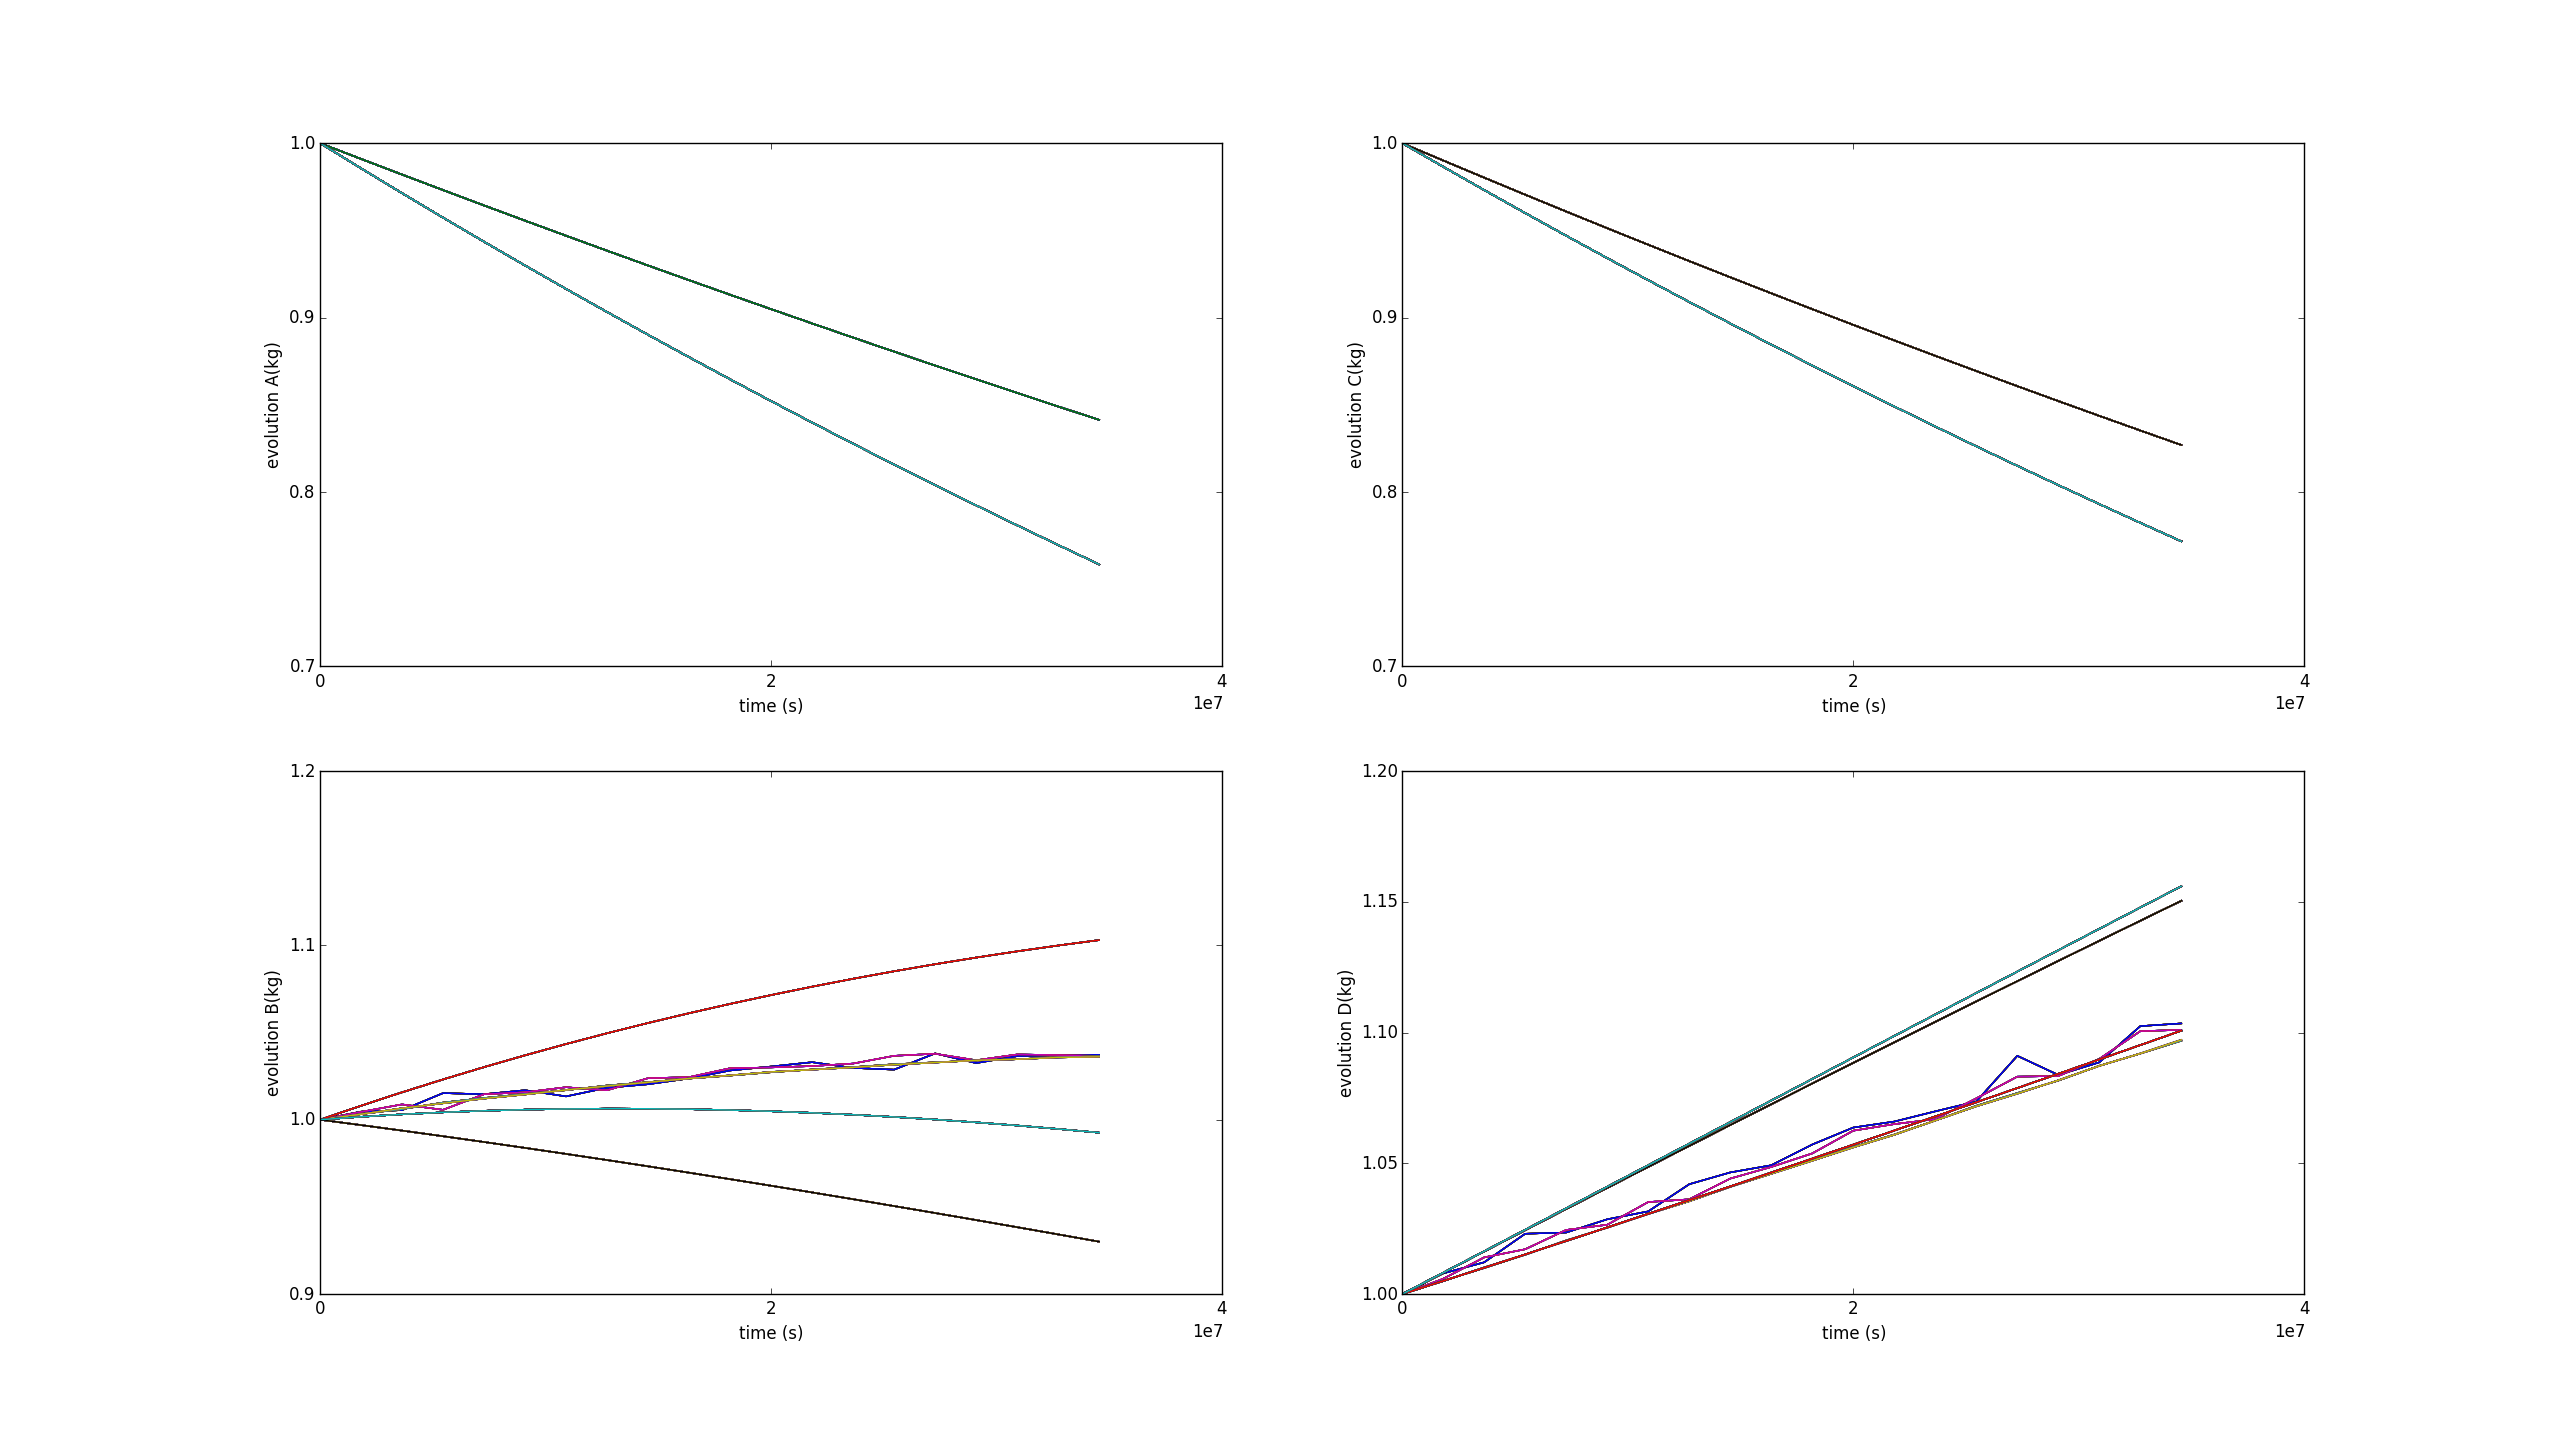
\includegraphics[scale=0.7]{pics/Grid_histories.png}
  \caption{Plot of the histories generated by the Grid sampling for variables $A,B,C,D$.}
  \label{fig:historiesGridPlotLine}
 \end{figure}
 %%%%%%%%%%%%%%%%%%%%%%%%%%%%%%%%%%%%%%%%%%%%%%%%%%%%%%%%%%
  In this block, both the Out-Stream types are constructed:
  \begin{itemize}
    \item \textit{Print}:
     \begin{itemize}
       \item named ``samples'' connected with the \textit{DataObjects} \textbf{Entity} ``samples''
                (\xmlNode{source})
       \item named ``histories'' connected with the \textit{DataObjects} \textbf{Entity} ``histories'' (\xmlNode{source}).
     \end{itemize}
      When these objects get used, all the information contained in the
      linked  \textit{DataObjects} are going
    to be exported in CSV files (\xmlNode{type}).
    \item \textit{Plot}:
    \begin{itemize}
      \item named ``historiesPlot'' connected with the  \textit{DataObjects}
      \textbf{Entity} ``samples''.  This plot will draw the final state of the
      variables $A,B,C,D$ with respect to the input variables $sigma$(s)
      and $decay$(s).
      \item named ``samplesPlot3D'' connected with the
      \textit{DataObjects} \textbf{Entity} ``histories''. This plot will draw the
      evolution of the variables $A,B,C,D$.
    \end{itemize}
     As it can be noticed, both plots are of type \textit{SubPlot}. Four plots
     are placed in each of the figures.
  \end{itemize}
   \item \textbf{\textit{Steps}}:
\begin{lstlisting}[style=XML,morekeywords={arg,extension,pauseAtEnd,overwrite}]
  <Steps>
    <MultiRun name="sample">
      <Input 	    class="Files" 			 type="input">referenceInput.xml</Input>
      <Model 	    class="Models" 		 type="Code">testModel</Model>
      <Sampler 	class="Samplers" 		 type="Grid">grid</Sampler>
      <Output 	class="DataObjects"  type="PointSet">samples</Output>
      <Output 	class="DataObjects"  type="HistorySet">histories</Output>
    </MultiRun>
    <IOStep name="writeHistories" pauseAtEnd="True">
        <Input class="DataObjects" type="HistorySet">histories</Input>
        <Input class="DataObjects" type="PointSet">samples</Input>
        <Output 	class="OutStreams" type="Plot">samplesPlot3D</Output>
        <Output 	class="OutStreams" type="Plot">historyPlot</Output>
        <Output 	class="OutStreams" type="Print">samples</Output>
        <Output 	class="OutStreams" type="Print">histories</Output>
    </IOStep>
  </Steps>
\end{lstlisting}
 %%%%%%%%%%%%%%%%%%%%%%%%%%%%%%%%%%%%%%%%%%%%%%%%%%%%%%%%%%
 %figure samples
 \begin{figure}[h!]
  \centering
  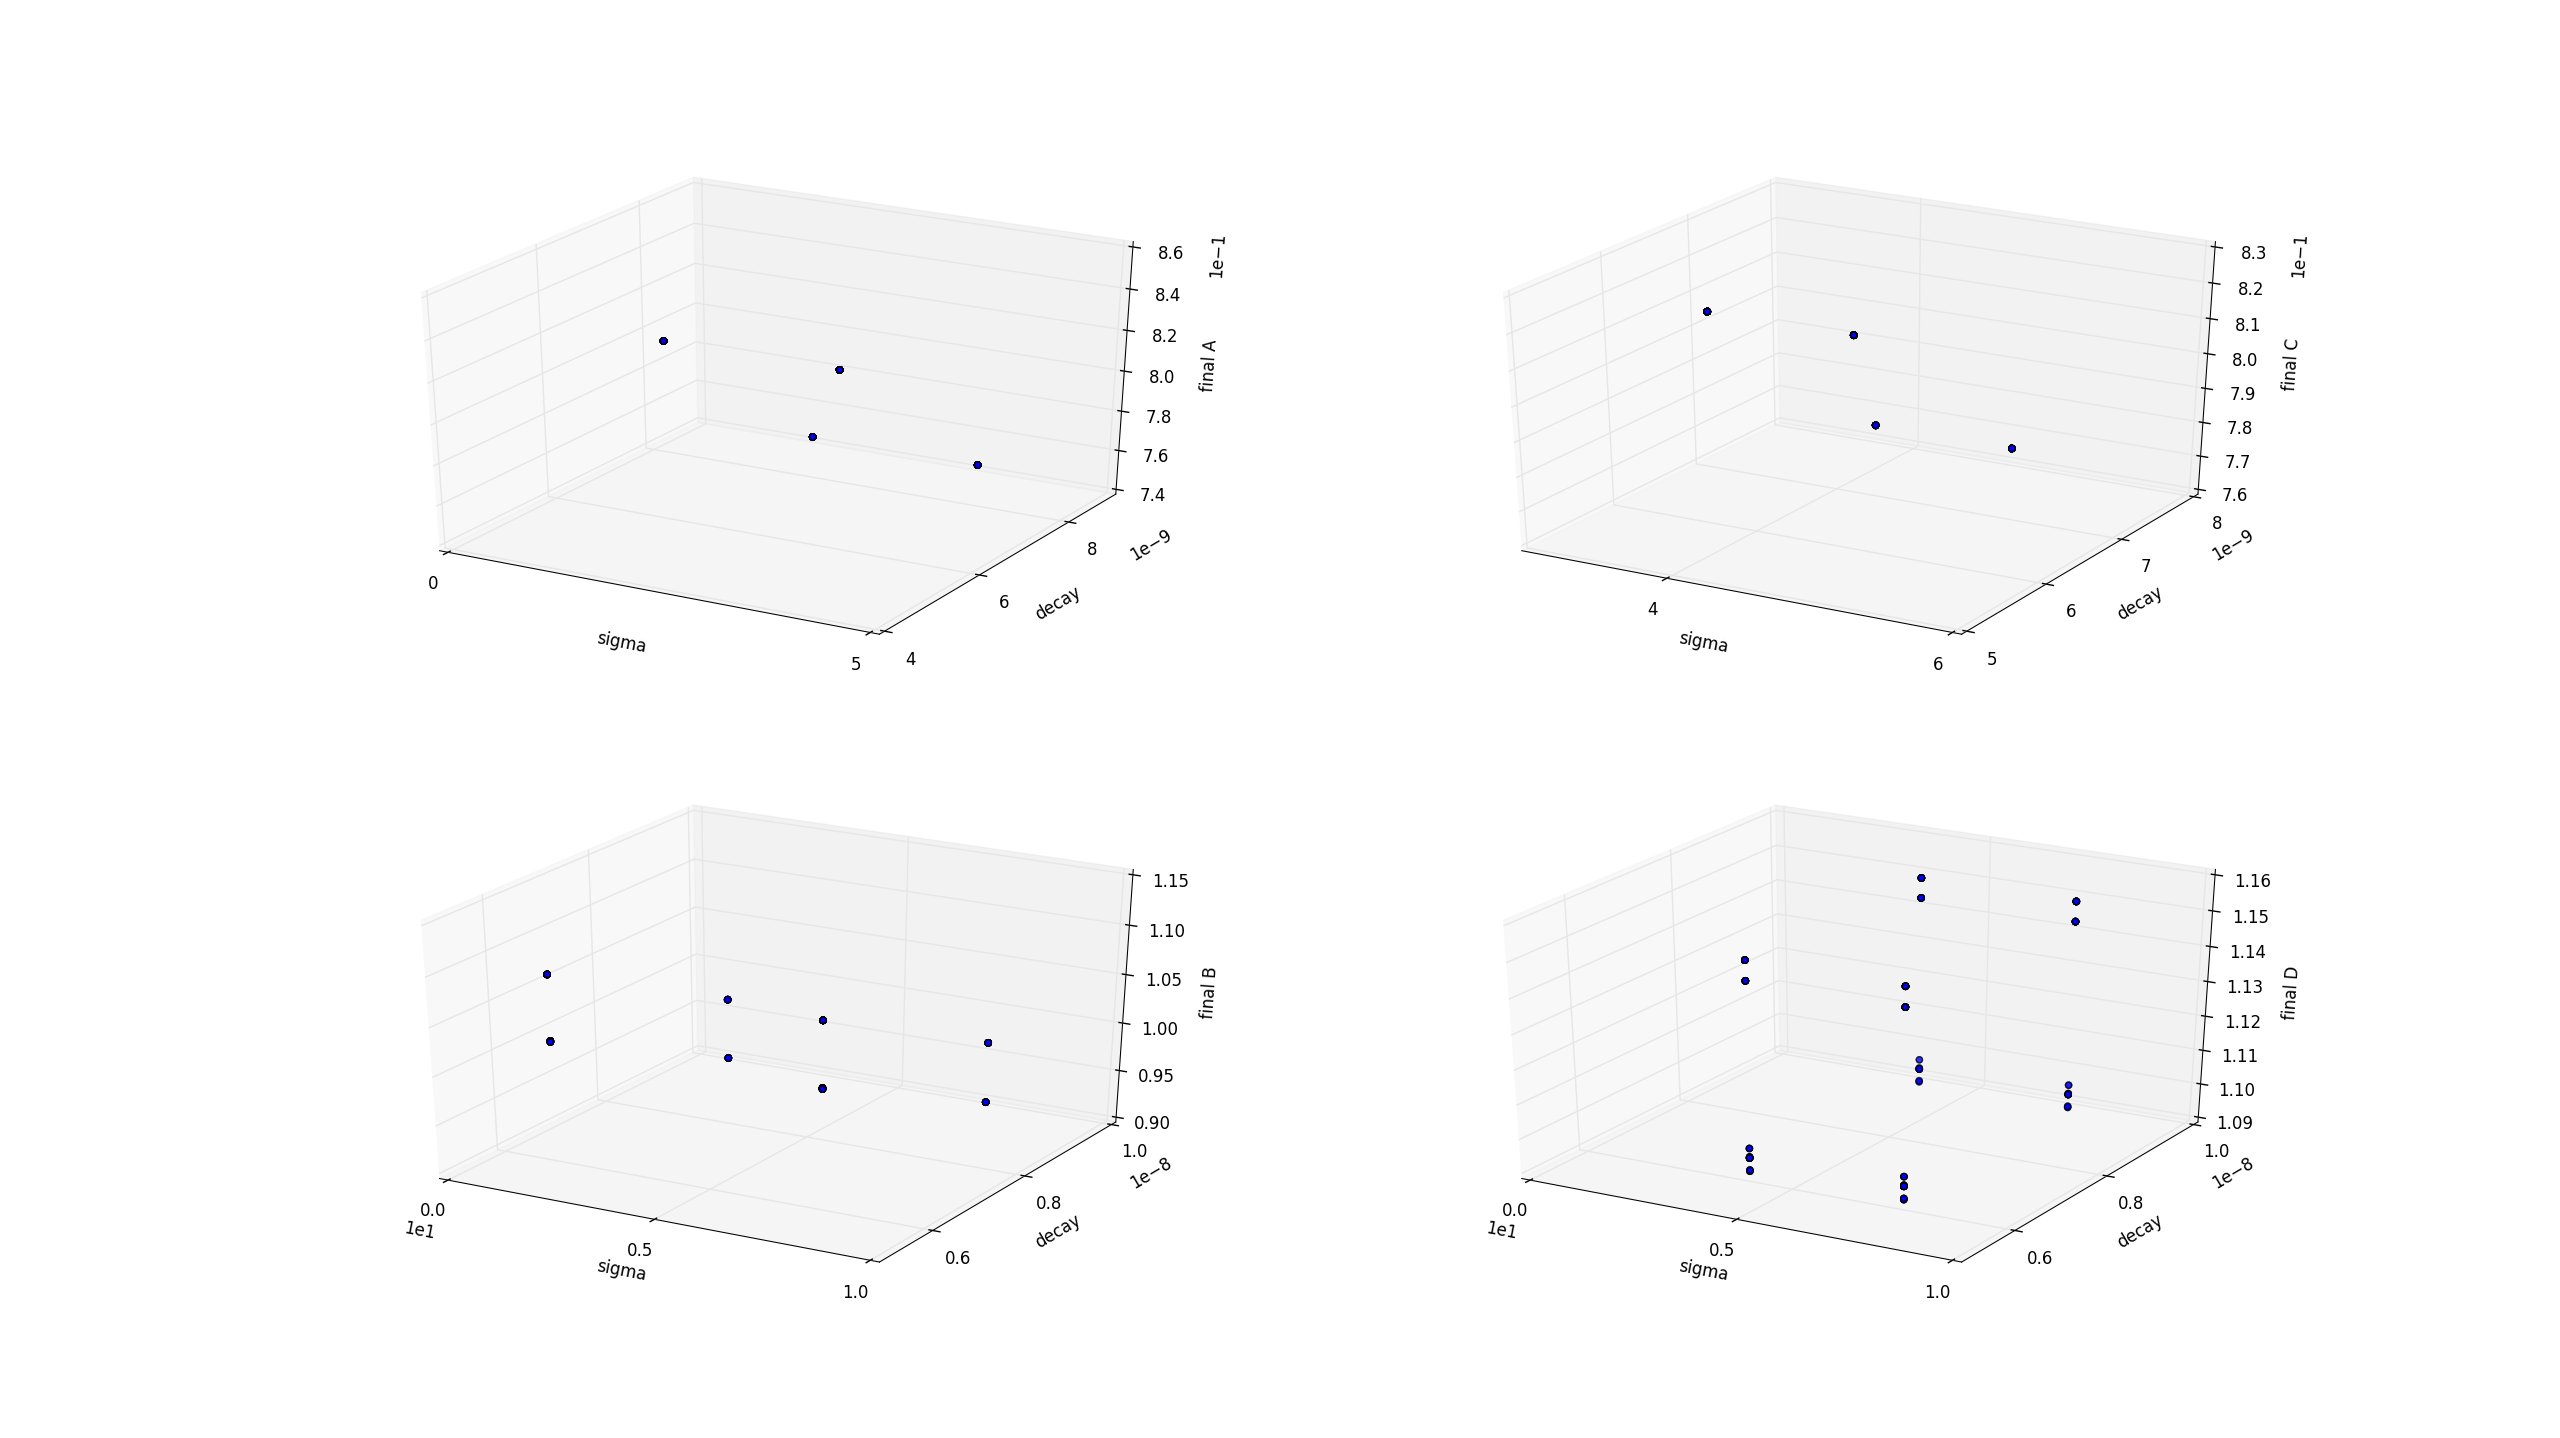
\includegraphics[scale=0.7]{pics/Grid_pointsets.png}
  \caption{Plot of the samples generated by the Grid sampling for variables $A,B,C,D$.}
  \label{fig:samplesGridPlotLine}
 \end{figure}
 %%%%%%%%%%%%%%%%%%%%%%%%%%%%%%%%%%%%%%%%%%%%%%%%%%%%%%%%%%
   Finally, all the previously defined \textbf{Entities} can be combined in
   the \xmlNode{Steps} block. As inferable,
   two \xmlNode{Steps} have been inputted:
   \begin{itemize}
     \item \xmlNode{MultiRun} named ``sample'', is used to run the multiple
     instances of the code and
     collect the outputs in the two \textit{DataObjects}. As it can be
     seen, the \xmlNode{Sampler} is inputted to communicate to the
     \textit{Step} that the driven code needs to
     be perturbed through the Grid sampling
     \item  \xmlNode{IOStep} named ``writeHistories'', used to 1) dump
     the ``histories'' and ``samples'' \textit{DataObjects}
     \textbf{Entity} in a CSV file and 2) plot the data in the PNG file and
     on the screen.
   \end{itemize}
\end{enumerate}
 Figures~\ref{fig:historiesGridPlotLine} and ~\ref{fig:samplesGridPlotLine}  report the evolution of the
 variables $A,B,C,D$ and their final values, respectively.

%%%%%%%%%%%%%%%%%%%%%%%%%
%%%%%%%%    STRATIFIED    %%%%%%%%
%%%%%%%%%%%%%%%%%%%%%%%%%
\subsection{Stratified}
\label{sub:Stratified}
The Stratified sampling is a class of methods that relies on the assumption that the input space (i.e.,uncertainties)
can be separated in regions (strata) based on similarity of the response of the system for input set within the
same strata. Following this assumption, the most rewarding (in terms of computational cost vs. knowledge gain)
sampling strategy would be to place one sample for each region. In this way, the same information is not
collected more than once and all the prototypical behavior are sampled at least once. In
Figure~\ref{fig:StratifiedSamplingExample}, the Stratified sampling approach is exemplified.
 \begin{figure}[h!]
  \centering
  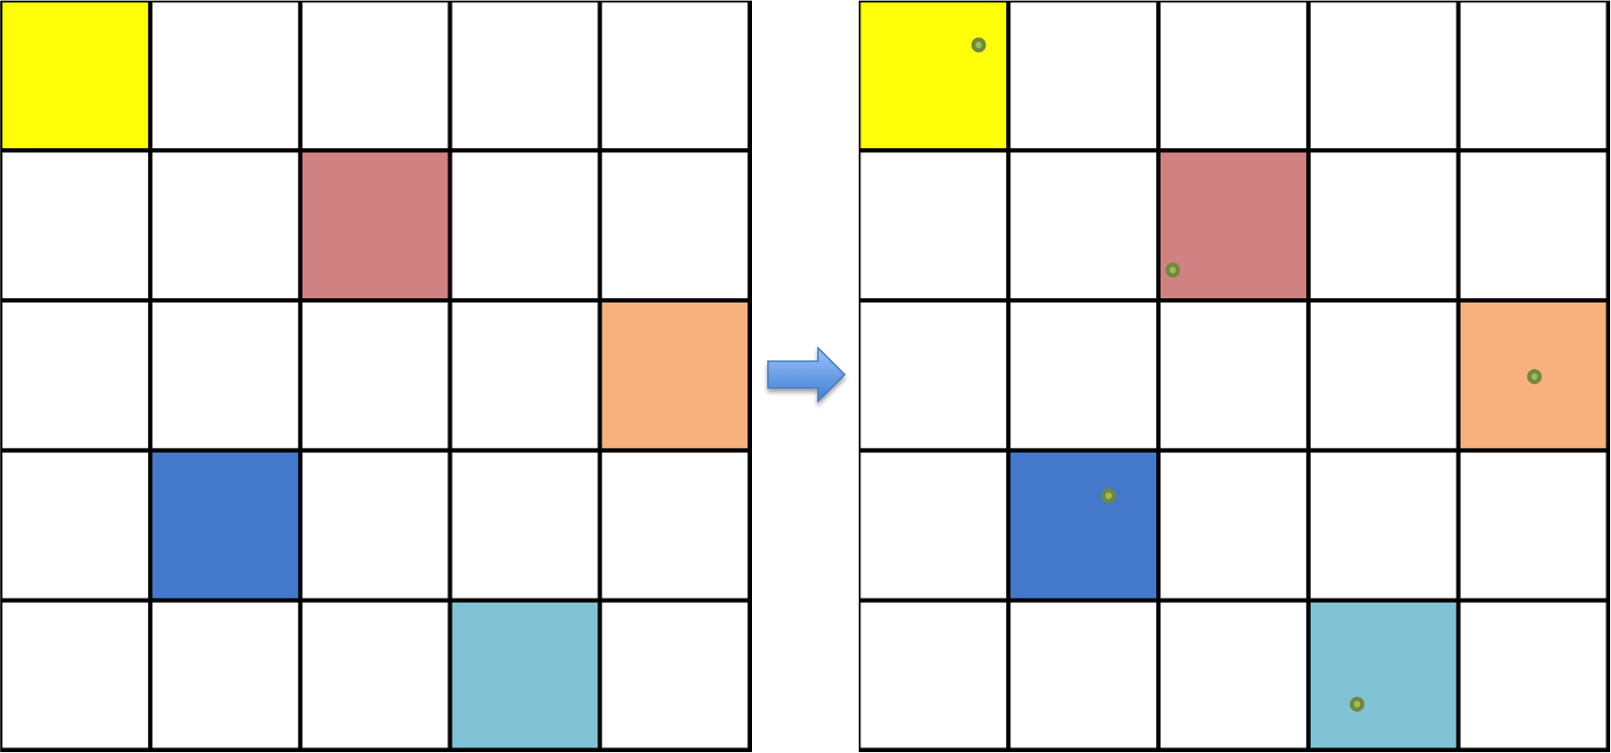
\includegraphics[scale=0.55]{pics/StratifiedSamplingExample.png}
  \caption{Example of Stratified sampling approach.}
  \label{fig:StratifiedSamplingExample}
 \end{figure}
\\In this section, a brief theoretical
background is reported. In addition,it is shown how to employ this methodology with RAVEN.
\subsubsection{Stratified theory introduction}
\label{subsub:Stratifiedtheory}
The Stratified sampling approach is a method for the exploration of the input space that consists of dividing the uncertain domain into subgroups before sampling. In the Stratified sampling, these subgroups must be:
\begin{itemize}
  \item Mutually exclusive: every element in the population must be assigned to only one stratum (subgroup)
  \item Collectively exhaustive: no population element can be excluded.
\end{itemize}
Then, simple random sampling or systematic sampling is applied within each stratum. The Latin Hyper-Cube sampling represents a specialized version of the stratified approach, when the domain strata are constructed in equally-probable CDF bins.
\\Similarly to what has been already reported for the Grid sampling, consider a set of  $m$ random variables $X_{j}, \, j=1,..,m$ having PDFs $pdf_{X_{j}}(x_{j})$ and, consequentially, CDF $cdf_{X_{j}}(x_{j})$ in the domain $\chi_{j}$. Then the expected value of a function $f$ of $X_{j}, \, j=1,..,m$ is as follows:
\begin{equation}
\begin{matrix}
\mathbb{E}(f(\overline{X})) =\sum f(x)   \prod_{j=1}^{m} pdf_{X_{j}}(x_{j}) & if \overline{X} \, discrete \\
\\
\mathbb{E}(f(\overline{X})) =\int f(x)\prod_{j=1}^{m} pdf_{X_{j}}(x_{j}) & \, if \overline{X} \, \, continuous
\end{matrix}
\end{equation}
In the Stratified approach, the domain of $\overline{X}$ is discretized in a set of strata. Consequentially, similarly to the Grid sampling, a weight needs to be associated with each realization in the input space:
\begin{equation}
\begin{matrix}
  w_{i}= \frac{\prod_{j=1}^{m} \left [  cdf_{X_{j}}(x_{i,j+1}) - cdf_{X_{j}}(x_{i,j}) \right ]}{\sum_{points}\prod_{j=1}^{m} \left [  cdf_{X_{j}}(x_{i,j+1}) - cdf_{X_{j}}(x_{i,j}) \right ]}
\end{matrix}
\end{equation}
Each realization carries a weight representative of each stratum.
\\Now consider
an $n-$strata of the domain of  $\overline{X}$, and compute the expected value of $f(x)$ over the discretization. Based on the previous equation, the computation of the expected value of $f(x)$ is as follows:
\begin{equation}
 \mathbb{E}(f(\overline{X})) \approx   \widetilde{f}_{n}(\overline{x}) = \frac{1}{\sum_{i=1}^{n}w_{i}} \sum_{i=1}^{n} f(\overline{x}_{i}) \times w_{i}
\end{equation}
\subsubsection{Stratified sampling through RAVEN}
\label{subsub:Stratifiedexample}
The goal of this section is to show how to:
 \begin{enumerate}
   \item Set up a simple Stratified sampling in order to perform a parametric analysis on a driven code
   \item Load the outputs of the code into the RAVEN DataObjects system
   \item Print out what contained in the DataObjects
   \item Generate basic plots of the code result.
\end{enumerate}
To accomplish these tasks, the following RAVEN \textbf{Entities} (XML blocks in the input files) are defined:
\begin{enumerate}
   \item \textbf{\textit{RunInfo}}:
\begin{lstlisting}[style=XML,morekeywords={arg,extension,pauseAtEnd,overwrite}]
  <RunInfo>
    <JobName>ChapterVII-I/Stratified</JobName>
    <Sequence>sample,writeHistories</Sequence>
    <WorkingDir>ChapterVII-I/Stratified</WorkingDir>
    <batchSize>12</batchSize>
  </RunInfo>
\end{lstlisting}
   As reported in Section~\ref{sub:EntitiesAndFlow}, the \textit{RunInfo} \textbf{Entity} is intended to set up the analysis
   that the user wants to perform. In this specific case, two steps (\xmlNode{Sequence}) are  run
   using 12 processors (\xmlNode{batchSize}). This means that
   12 instances of the driven code are run simultaneously.
   Every time a simulation ends, a new one is launched.
   \item \textbf{\textit{Files}}:
\begin{lstlisting}[style=XML,morekeywords={arg,extension,pauseAtEnd,overwrite}]
  <Files>
    <Input name="referenceInput.xml" type="input">referenceInput.xml</Input>
  </Files>
\end{lstlisting}
   Since the considered code uses a single input file, in this section the original input is placed.
   The attribute  \xmlAttr{name} represents the alias that is going to be used in all the other input blocks in order to refer to this file.
   \item \textbf{\textit{Models}}:
\begin{lstlisting}[style=XML,morekeywords={arg,extension,pauseAtEnd,overwrite}]
   <Models>
      <Code name="testModel" subType="GenericCode">
        <executable>
    ../physicalCode/analyticalbateman/AnalyticalDplMain.py
        </executable>
        <clargs arg="python" type="prepend"/>
        <clargs arg="" extension=".xml" type="input"/>
        <clargs arg="" extension=".csv" type="output"/>
        <prepend>python</prepend>
      </Code>
    <Models>
\end{lstlisting}
 The Model here is represented by the
 \textbf{AnalyticalBateman}, which already dumps its output file in a
 CSV format (standard format that RAVEN can read). For this reason,
 the \textit{GenericCode} interface is used.
   \item \textbf{\textit{Distributions}}:
\begin{lstlisting}[style=XML,morekeywords={arg,extension,pauseAtEnd,overwrite}]
  <Distributions>
      <Uniform name="sigma">
          <lowerBound>1</lowerBound>
          <upperBound>10</upperBound>
      </Uniform>
      <Uniform name="decayConstant">
          <lowerBound>0.000000005</lowerBound>
          <upperBound>0.000000010</upperBound>
      </Uniform>
  </Distributions>
\end{lstlisting}
  In the Distributions XML section, the stochastic model for the
  uncertainties  treated by the Stratified sampling are reported. In
  this case two distributions are defined:
  \begin{itemize}
    \item $sigma \sim \mathbb{U}(1,10)$, used to model the uncertainties
    associated with  the Model \textit{sigma}(s)
    \item  $decayConstant \sim \mathbb{U}(0.5e-8,1e-8)$,  used to
    model the uncertainties
    associated with  the Model \textit{decay constants}.
  \end{itemize}
   \item \textbf{\textit{Samplers}}:
\begin{lstlisting}[style=XML,morekeywords={arg,extension,pauseAtEnd,overwrite}]
    <Stratified name="stratified">
      <variable name="sigma-A">
        <distribution>sigma</distribution>
        <grid construction="equal" steps="100" type="value">2 4.0</grid>
      </variable>
      <variable name="decay-A">
        <distribution>decayConstant</distribution>
        <grid construction="equal" steps="100" type="value">0.000000005 0.000000008</grid>
      </variable>
      <variable name="sigma-B">
          <distribution>sigma</distribution>
          <grid construction="equal" steps="100" type="CDF">0.1 0.8</grid>
      </variable>
      <variable name="decay-B">
          <distribution>decayConstant</distribution>
          <grid construction="equal" steps="100" type="CDF">0.1 0.8</grid>
      </variable>
      <variable name="sigma-C">
          <distribution>sigma</distribution>
          <grid construction="equal" steps="100" type="value">1.0 5</grid>
      </variable>
      <variable name="decay-C">
          <distribution>decayConstant</distribution>
          <grid construction="equal" steps="100" type="CDF">0.1 0.5</grid>
      </variable>
      <variable name="sigma-D">
          <distribution>sigma</distribution>
          <grid construction="equal" steps="100" type="CDF">0.4 0.8</grid>
      </variable>
      <variable name="decay-D">
          <distribution>decayConstant</distribution>
          <grid construction="equal" steps="100" type="CDF">0.1 0.8</grid>
      </variable>
    </Stratified>
\end{lstlisting}
  To employ the Stratified sampling strategy, a
  \xmlNode{Stratified} node needs to be specified. In each variable section, the  \xmlNode{grid} is defined.
  It is important to mention that the number of \xmlAttr{steps} needs to be the same for each of the variables,
  since, as reported in previous section, the Stratified sampling strategy it discretizes the domain in strata.
  The number of samples finally requested is equal to $n_{samples} = n_{steps} = 100$.
  If the grid for each variables is defined in CDF and of  \xmlAttr{type} = ``equal'', the Stratified
  sampling corresponds to the well-known Latin Hyper Cube sampling.
   \item \textbf{\textit{DataObjects}}:
\begin{lstlisting}[style=XML,morekeywords={arg,extension,pauseAtEnd,overwrite}]
  <DataObjects>
    <PointSet name="samples">
      <Input>
        sigma-A,sigma-B,sigma-C,sigma-D,
        decay-A,decay-B,decay-C,decay-D
      </Input>
      <Output>A,B,C,D,time</Output>
    </PointSet>
    <HistorySet name="histories">
        <Input>
          sigma-A,sigma-B,sigma-C,sigma-D,
          decay-A,decay-B,decay-C,decay-D
        </Input>
        <Output>A,B,C,D,time</Output>
    </HistorySet>
  </DataObjects>
\end{lstlisting}
  In this block, two \textit{DataObjects} are defined: 1) PointSet named
  ``samples'', 2) HistorySet named ``histories''.
  In the \xmlNode{Input} node all the variables
  perturbed through the Stratified strategy are listed. In this way, any
  realization in the input space is linked to the outputs listed in  the
  \xmlNode{Output} node.
   \item \textbf{\textit{OutStreams}}:
\begin{lstlisting}[style=XML,morekeywords={arg,extension,pauseAtEnd,overwrite}]
  <OutStreams>
    <Print name="samples">
      <type>csv</type>
      <source>samples</source>
    </Print>
    <Print name="histories">
      <type>csv</type>
      <source>histories</source>
    </Print>
    <Plot dim="2" name="historiesPlot" overwrite="false" verbosity="debug">
        <plotSettings>
            <gridSpace>2 2</gridSpace>
            <plot>
                <type>line</type>
                <x>histories|Output|time</x>
                <y>histories|Output|A</y>
                <color>blue</color>
                <gridLocation>
                  <x>0</x>
                  <y>0</y>
                </gridLocation>
                <xlabel>time (s)</xlabel>
                <ylabel>evolution A(kg)</ylabel>
            </plot>
            <plot>
                <type>line</type>
                <x>histories|Output|time</x>
                <y>histories|Output|B</y>
                <color>red</color>
                <gridLocation>
                    <x>1</x>
                    <y>0</y>
                </gridLocation>
                <xlabel>time (s)</xlabel>
                <ylabel>evolution B(kg)</ylabel>
            </plot>
            <plot>
                <type>line</type>
                <x>histories|Output|time</x>
                <y>histories|Output|C</y>
                <color>yellow</color>
                <gridLocation>
                    <x>0</x>
                    <y>1</y>
                </gridLocation>
                <xlabel>time (s)</xlabel>
                <ylabel>evolution C(kg)</ylabel>
            </plot>
            <plot>
                <type>line</type>
                <x>histories|Output|time</x>
                <y>histories|Output|D</y>
                <color>black</color>
                <gridLocation>
                    <x>1</x>
                    <y>1</y>
                </gridLocation>
                <xlabel>time (s)</xlabel>
                <ylabel>evolution D(kg)</ylabel>
            </plot>
        </plotSettings>
        <actions>
            <how>png,screen</how>
            <title>
                <text> </text>
            </title>
        </actions>
    </Plot>
    <Plot dim="3" name="samplesPlot3D" overwrite="false" verbosity="debug">
        <plotSettings>
            <gridSpace>2 2</gridSpace>
            <plot>
                <type>scatter</type>
                <x>samples|Input|sigma-A</x>
                <y>samples|Input|decay-A</y>
                <z>samples|Output|A</z>
                <color>blue</color>
                <gridLocation>
                  <x>0</x>
                  <y>0</y>
                </gridLocation>
                <xlabel>sigma</xlabel>
                <ylabel>decay</ylabel>
                <zlabel>final A</zlabel>
            </plot>
            <plot>
                <type>scatter</type>
                <x>samples|Input|sigma-B</x>
                <y>samples|Input|decay-B</y>
                <z>samples|Output|B</z>
                <color>red</color>
                <gridLocation>
                    <x>1</x>
                    <y>0</y>
                </gridLocation>
                <xlabel>sigma</xlabel>
                <ylabel>decay</ylabel>
                <zlabel>final B</zlabel>
            </plot>
            <plot>
                <type>scatter</type>
                <type>scatter</type>
                <x>samples|Input|sigma-C</x>
                <y>samples|Input|decay-C</y>
                <z>samples|Output|C</z>
                <color>yellow</color>
                <gridLocation>
                    <x>0</x>
                    <y>1</y>
                </gridLocation>
                <xlabel>sigma</xlabel>
                <ylabel>decay</ylabel>
                <zlabel>final C</zlabel>
            </plot>
            <plot>
                <type>scatter</type>
                <x>samples|Input|sigma-D</x>
                <y>samples|Input|decay-D</y>
                <z>samples|Output|D</z>
                <color>black</color>
                <gridLocation>
                    <x>1</x>
                    <y>1</y>
                </gridLocation>
                <xlabel>sigma</xlabel>
                <ylabel>decay</ylabel>
                <zlabel>final D</zlabel>
            </plot>
            <xlabel>sigma</xlabel>
            <ylabel>decay</ylabel>
            <zlabel>final response</zlabel>
        </plotSettings>
        <actions>
            <how>png,screen</how>
            <title>
                <text> </text>
            </title>
        </actions>
    </Plot>
  </OutStreams>
\end{lstlisting}
 %%%%%%%%%%%%%%%%%%%%%%%%%%%%%%%%%%%%%%%%%%%%%%%%%%%%%%%%%%
 %figure histories
 \begin{figure}[h!]
  \centering
  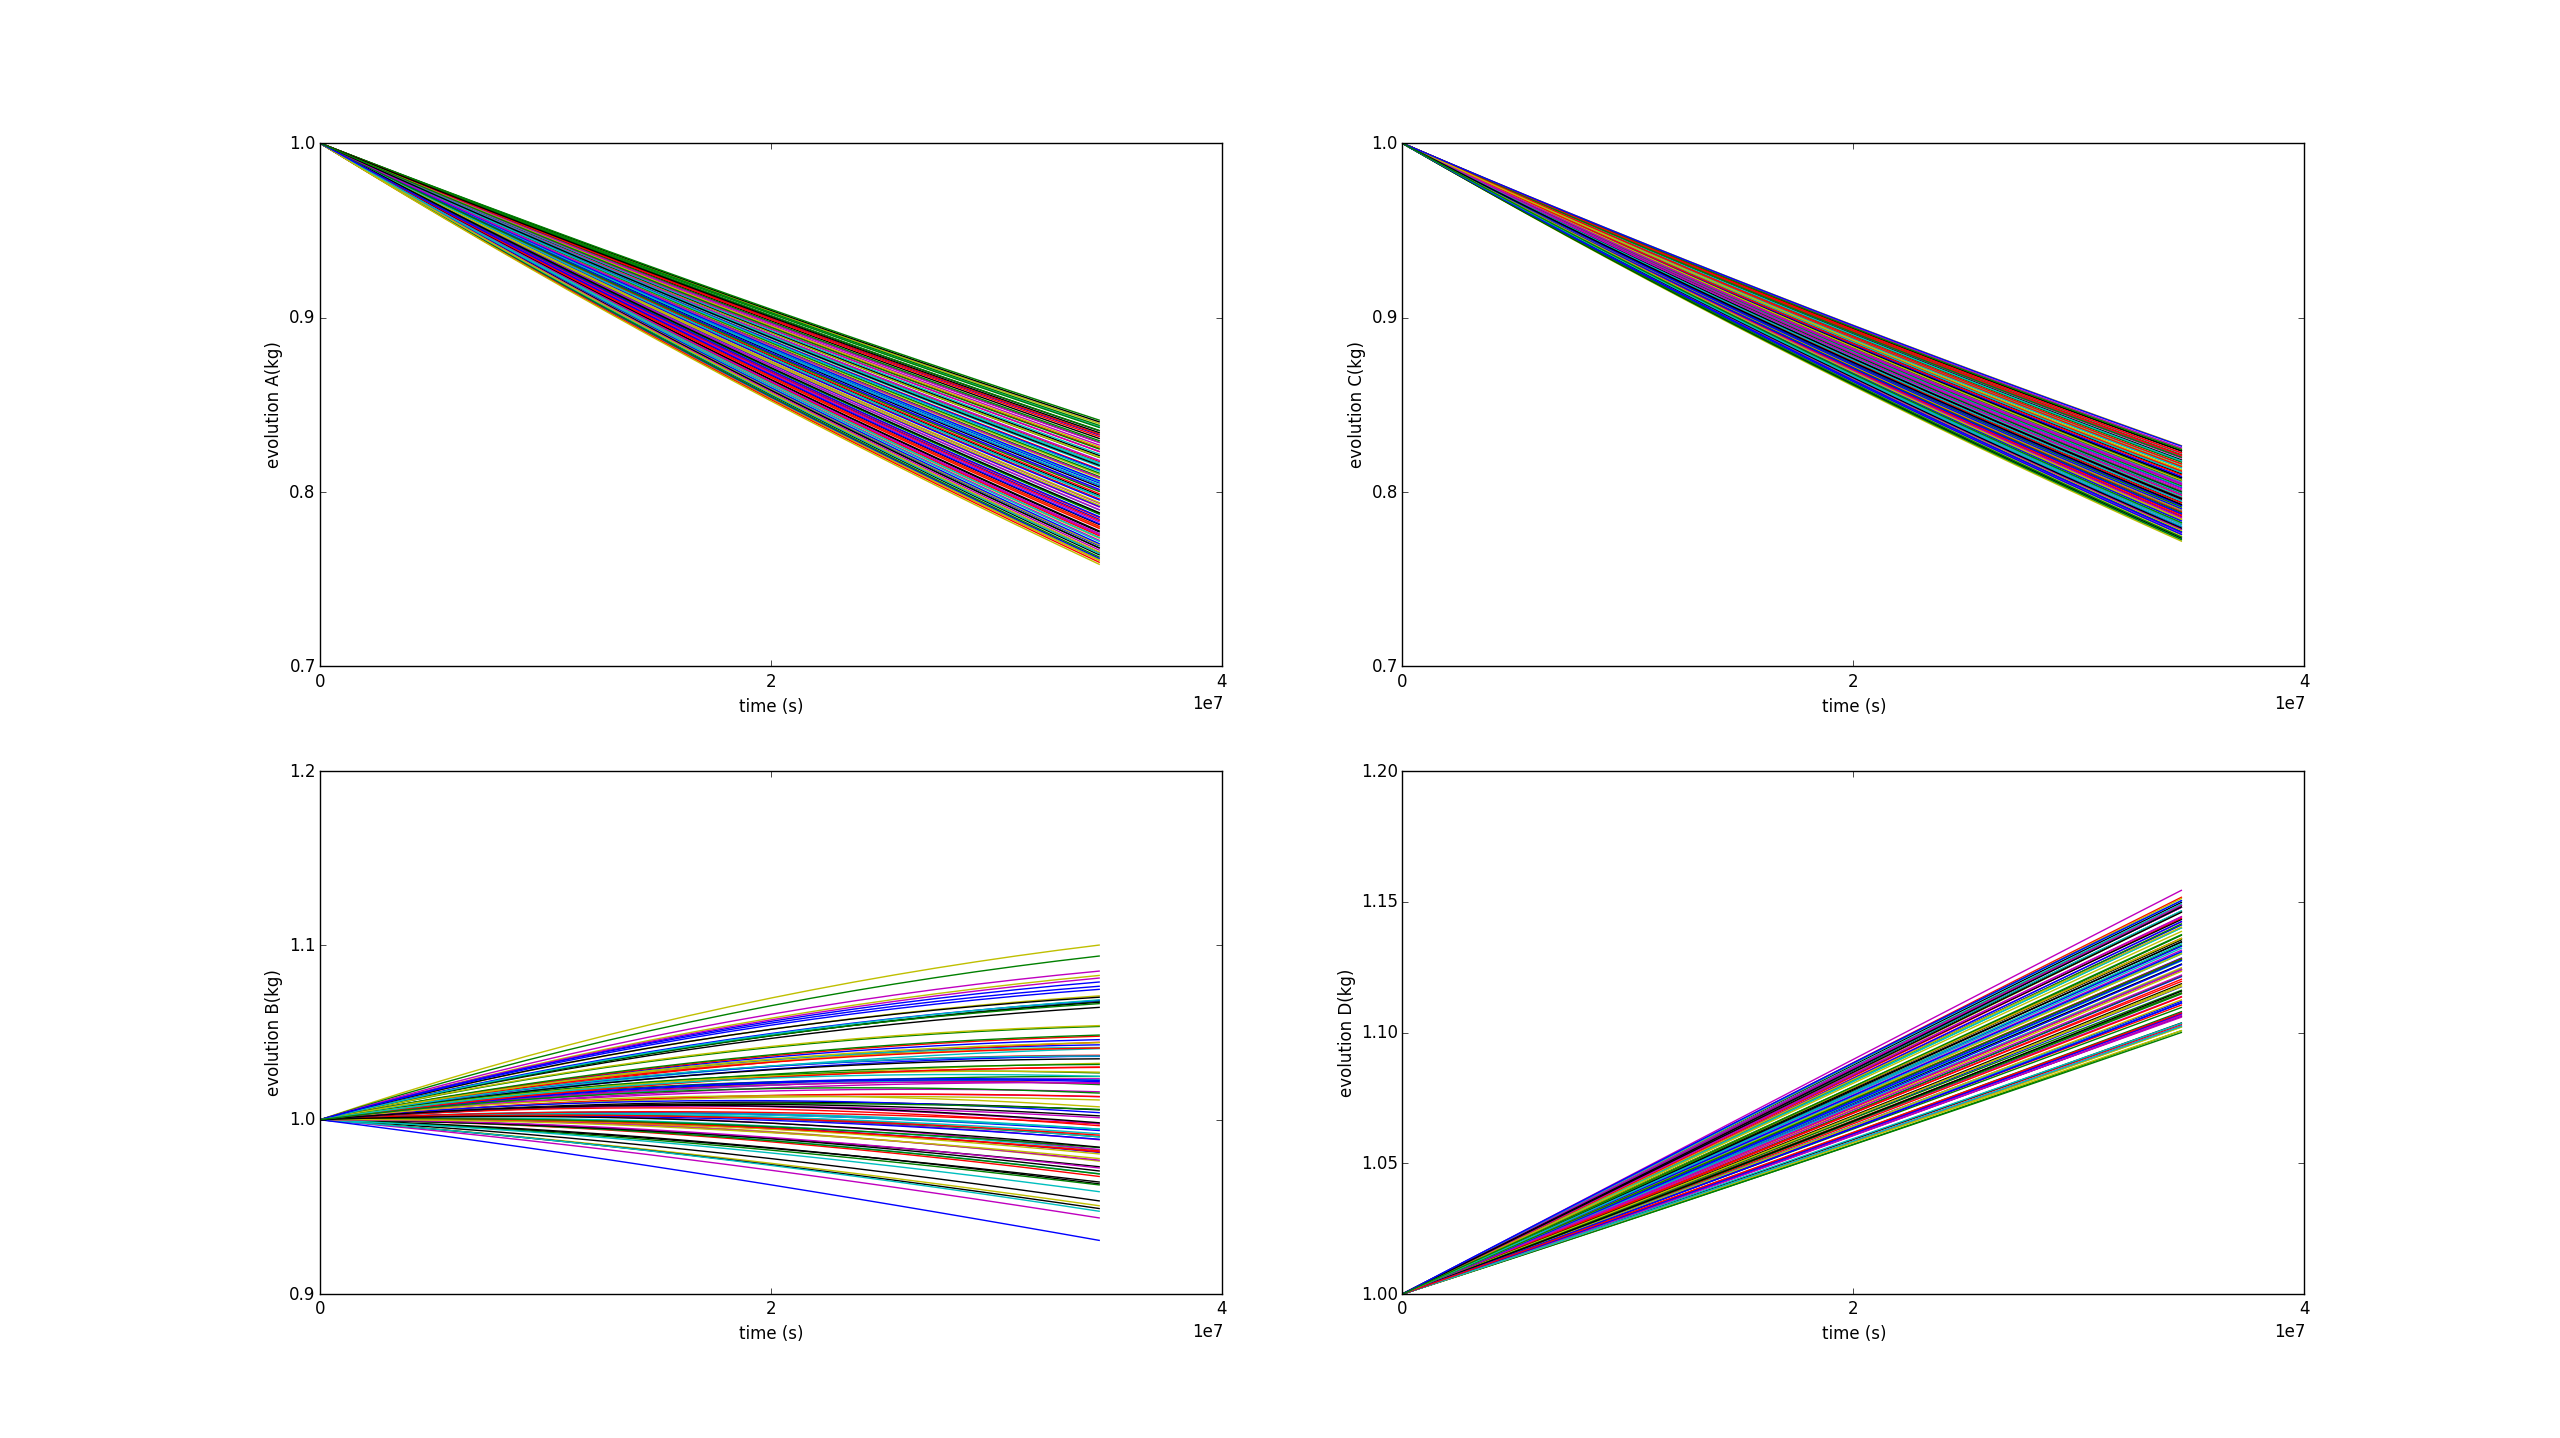
\includegraphics[scale=0.7]{pics/Stratified_histories.png}
  \caption{Plot of the histories generated by the Stratified sampling for variables $A,B,C,D$.}
  \label{fig:historiesStratifiedPlotLine}
 \end{figure}
 %%%%%%%%%%%%%%%%%%%%%%%%%%%%%%%%%%%%%%%%%%%%%%%%%%%%%%%%%%
  In this block, both the Out-Stream types are constructed:
  \begin{itemize}
    \item \textit{Print}:
     \begin{itemize}
       \item named ``samples'' connected with the \textit{DataObjects} \textbf{Entity} ``samples''
                (\xmlNode{source})
       \item named ``histories'' connected with the \textit{DataObjects} \textbf{Entity} ``histories'' (\xmlNode{source}).
     \end{itemize}
      When these objects get used, all the information contained in the
      linked  \textit{DataObjects} are going
    to be exported in CSV files (\xmlNode{type}).
    \item \textit{Plot}:
    \begin{itemize}
      \item named ``historiesPlot'' connected with the  \textit{DataObjects}
      \textbf{Entity} ``samples''.  This plot will draw the final state of the
      variables $A,B,C,D$ with respect to the input variables $sigma$(s)
      and $decay$(s)
      \item named ``samplesPlot3D'' connected with the
      \textit{DataObjects} \textbf{Entity} ``histories''. This plot will draw the
      evolution of the variables $A,B,C,D$.
    \end{itemize}
     As it can be noticed, both plots are of type \textit{SubPlot}. Four plots
     are going to be placed in each of the figures.
  \end{itemize}
   \item \textbf{\textit{Steps}}:
\begin{lstlisting}[style=XML,morekeywords={arg,extension,pauseAtEnd,overwrite}]
  <Steps>
    <MultiRun name="sample">
      <Input 	    class="Files" 			 type="input">referenceInput.xml</Input>
      <Model 	    class="Models" 		 type="Code">testModel</Model>
      <Sampler 	class="Samplers" 		 type="Stratified">stratified</Sampler>
      <Output 	class="DataObjects"  type="PointSet">samples</Output>
      <Output 	class="DataObjects"  type="HistorySet">histories</Output>
    </MultiRun>
    <IOStep name="writeHistories" pauseAtEnd="True">
        <Input class="DataObjects" type="HistorySet">histories</Input>
        <Input class="DataObjects" type="PointSet">samples</Input>
        <Output 	class="OutStreams" type="Plot">samplesPlot3D</Output>
        <Output 	class="OutStreams" type="Plot">historyPlot</Output>
        <Output 	class="OutStreams" type="Print">samples</Output>
        <Output 	class="OutStreams" type="Print">histories</Output>
    </IOStep>
  </Steps>
\end{lstlisting}
 %%%%%%%%%%%%%%%%%%%%%%%%%%%%%%%%%%%%%%%%%%%%%%%%%%%%%%%%%%
 %figure samples
 \begin{figure}[h!]
  \centering
  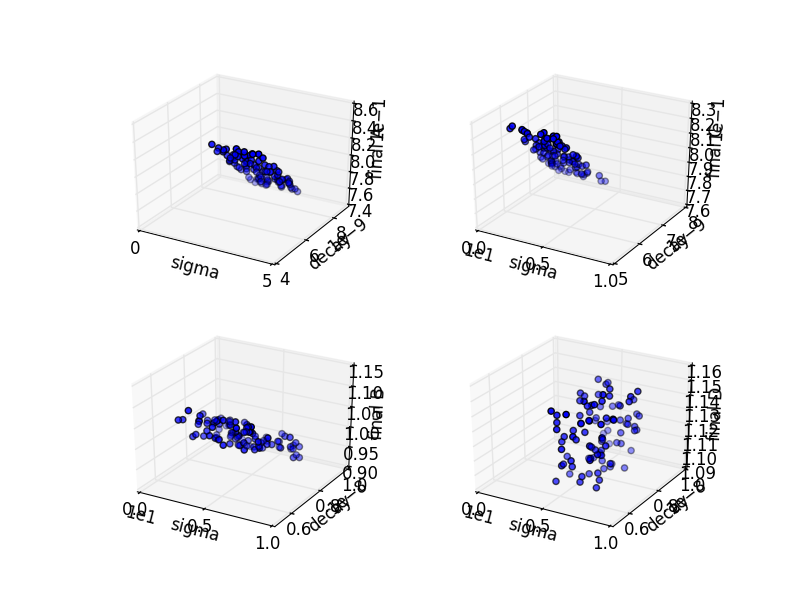
\includegraphics[scale=0.7]{pics/Stratified_pointsets.png}
  \caption{Plot of the samples generated by the Stratified sampling for variables $A,B,C,D$.}
  \label{fig:samplesStratifiedPlotLine}
 \end{figure}
 %%%%%%%%%%%%%%%%%%%%%%%%%%%%%%%%%%%%%%%%%%%%%%%%%%%%%%%%%%
   Finally, all the previously defined \textbf{Entities} can be combined in
   the \xmlNode{Steps} block. As inferable,
   two \xmlNode{Steps} have been inputted:
   \begin{itemize}
     \item \xmlNode{MultiRun} named ``sample'', used to run the multiple
     instances of the driven code and
     collect the outputs in the two \textit{DataObjects}. As it can be
     seen, the \xmlNode{Sampler} is inputted to communicate to the
     \textit{Step} that the driven code needs to
     be perturbed through the Stratified sampling.
     \item  \xmlNode{IOStep} named ``writeHistories'', used to 1) dump
     the ``histories'' and ``samples'' \textit{DataObjects}
     \textbf{Entity} in a CSV file and 2) plot the data in the PNG file and
     on the screen.
   \end{itemize}
\end{enumerate}
 As previously mentioned, Figures~\ref{fig:historiesStratifiedPlotLine} and ~\ref{fig:samplesStratifiedPlotLine}  report the evolution of the
 variables $A,B,C,D$ and their final values, respectively.

%%%%%%%%%%%%%%%%%%%%%%%%%

\subsection{Sparse Grid Collocation}
\label{sub:SGC}
The Sparse Grid Collocation sampler represents an advanced methodology to perform Uncertainty Quantification. They aim
to explore the input space leveraging the information contained in the associated probability density functions. It builds on generic Grid sampling by selecting evaluation points based on characteristic quadratures as part of stochastic collocation for generalized polynomial chaos uncertainty quantification. In collocation an N-D grid is constructed, with each uncertain variable providing an axis. Along each axis, the points of evaluation correspond to quadrature points necessary to integrate polynomials. In the simplest (and most naive) case, a N-D tensor product of all possible combinations of points from each dimension’s quadrature is constructed as sampling points. The number of necessary samples can be reduced by employing Smolyak-like sparse grid algorithms, which use reduced combinations of polynomial orders to reduce the necessary sampling space.
\\In this Section, a brief theoretical
background is reported. In addition, it is shown how to employ this methodology with RAVEN.
\subsubsection{Sparse Grid Collocation Theory Introduction}
\label{subsub:SGctheory}
\paragraph{Generalized Polynomial Chaos}
In general, polynomial chaos expansion (PCE) methods seek to interpolate the simulation code as a combination of
polynomials of varying degree in each dimension of the input space.  Originally Wiener
proposed expanding in Hermite polynomials for Gaussian-normal distributed variables~\cite{wiener}.  Askey and
Wilson generalized Hermite polynomials to include Jacobi polynomials, including Legendre and Laguerre
polynomials~\cite{Wiener-Askey}.  Xiu and Karniadakis combines these concepts to perform PCE for a range of Gaussian-based
distributions with corresponding polynomials,
including Legendre polynomials for uniform distributions, Laguerre polynomials for Gamma distributions, and
Jacobi polynomials for Beta distributions \cite{xiu}.

In each of these cases, a probability-weighted
integral over the distribution can be cast in a way that the corresponding polynomials are orthogonal over the
same weight and interval.  These chaos Wiener-Askey polynomials were used by Xiu and Karniadakis to develop
the generalized polynomial chaos expansion method (gPC), including a transformation for applying the same
method to arbitrary distributions (as long as they have a known inverse CDF)~\cite{xiu}.  Two significant
methodologies have grown from gPC application.  The first makes use of Lagrange polynomials to expand the
original function or simulation code, as they can be made orthogonal over the same domain as the
distributions~\cite{SCLagrange}; the other uses the Wiener-Askey polynomials~\cite{xiu}.

Consider a simulation code that produces a quantity of interest $u$ as a function $u(Y)$ whose arguments are
the uncertain, distributed input
parameters $Y=(Y_1,\ldots,Y_n,\ldots,Y_N)$.  A particular realization $\omega$ of $Y_n$ is expressed by
$Y_n(\omega)$, and a single realization of the entire input space results in a solution to the function as
$u(Y(\omega))$. Obtaining a realization of $u(Y)$ may take considerable computation time and
effort.
$u(Y)$ gets expanded in orthonormal multidimensional polynomials $\Phi_k(Y)$, where $k$ is a multi-index tracking
the polynomial order in each axis of the polynomial Hilbert space, and $\Phi_k(Y)$ is constructed as
\begin{equation}\label{eq:gPC}
  \Phi_k(Y) = \prod_{n=1}^N \phi_{k_n}(Y_n),
\end{equation}
where $\phi_{k_n}(Y_n)$ is a single-dimension Wiener-Askey orthonormal polynomial of order $k_n$ and
$k=(k_1,\ldots,k_n,\ldots,k_N)$, $k_n\in\mathbb{N}^0$.  For example, given $u(y_1,y_2,y_3)$, $k=(2,1,4)$
is the multi-index of the
product of a second-order polynomial in $y_1$, a first-order polynomial in $y_2$, and a fourth-order
polynomial in $y_4$. The gPC for $u(Y)$ using this notation is
\begin{equation}
  u(Y) \approx \sum_{k\in\Lambda(L)} u_k\Phi_k(Y),
\end{equation}
where $u_k$ is a scalar weighting polynomial coefficient. The polynomials used in the expansion are determined
by the set of multi-indices $\Lambda(L)$, where $L$ is a truncation order.  In the limit
that $\Lambda$ contains all possible combinations of polynomials of any order, Eq. \ref{eq:gPC} is exact.
Practically, however, $\Lambda$ is truncated to some finite set of combinations, discussed in section
\ref{sec:indexSets}.

Using the orthonormal properties of the Wiener-Askey polynomials,
\begin{equation}
  \int_\Omega \Phi_k(Y)\Phi_{\hat k}(Y) \rho(Y) dY = \delta_{k\hat k},
\end{equation}
where $\rho(Y)$ is the combined PDF of $Y$, $\Omega$ is the multidimensional domain of $Y$, and $\delta_{nm}$
is the Dirac delta, an expression of the polynomial expansion coefficients can be isolated.
We multiply both sides of Eq. \ref{eq:gPC} by
$\Phi_{\hat k}(Y)$, integrate both sides over the probability-weighted input domain, and sum over all $\hat k$
to obtain the coefficients, sometimes referred to as polynomial expansion moments,
\begin{align}\label{eq:polycoeff}
  u_k &= \frac{\langle u(Y)\Phi_k(Y) \rangle}{\langle \Phi_k(Y)^2 \rangle},\\
      &= \langle u(Y)\Phi_k(Y) \rangle,
\end{align}
where we use the angled bracket notation to denote the probability-weighted inner product,
\begin{equation}
  \langle f(Y) \rangle \equiv \int_\Omega f(Y)\rho(Y) dY.
\end{equation}
When $u(Y)$ has an analytic form, these coefficients can be solved by integration; however, in general other
methods must be applied to numerically perform the integral.  While tools such as Monte Carlo integration can
be used to evaluate the integral, the properties of Gaussian quadratures, because of the
probability weights and domain, can be harnessed.  This stochastic collocation method is discussed in section \ref{sec:stoch
coll}.
\paragraph{Polynomial Index Set Construction}\label{sec:indexSets}
The main concern in expanding a function in interpolating multidimensional polynomials is choosing appropriate polynomials to
make up the expansion.
There are many generic ways by which a polynomial set can be constructed.  Here  three static
approaches are presented:
\begin{itemize}
  \item Tensor Product
  \item Total Degree
  \item Hyperbolic Cross.
\end{itemize}
In the nominal tensor
product case, $\Lambda(L)$ contains all possible combinations of polynomial indices up to truncation order $L$ in each
dimension, as:
\begin{equation}
  \Lambda_\text{TP}(L)=\Big\{\bar p=(p_1,\cdots,p_N): \max_{1\leq n\leq N}p_n\leq L
\Big\}.
\end{equation}
The cardinality of this index set is $|\Lambda_\text{TP}(L)|=(L+1)^N$. For example, for a two-dimensional
input space ($N$=2) and truncation limit $L=3$, the index set $\Lambda_\text{TP}(3)$ is given in Table
\ref{tab:TP}, where the notation $(1,2)$ signifies the product of a polynomial that is first order in $Y_1$
and second order in $Y_2$.

\begin{table}[h]
  \centering
  \begin{tabular}{c c c c}
    (3,0) & (3,1) & (3,2) & (3,3) \\
    (2,0) & (2,1) & (2,2) & (2,3) \\
    (1,0) & (1,1) & (1,2) & (1,3) \\
    (0,0) & (0,1) & (0,2) & (0,3)
  \end{tabular}
  \caption{Tensor Product Index Set, $N=2,L=3$.}
  \label{tab:TP}
\end{table}

It is evident there is some inefficiencies in this index set.  First, it suffers dramatically from the
\emph{curse of dimensionality}; that is, the number of polynomials required grows exponentially with
increasing dimensions.  Second, the total order of polynomials is not considered.  Assuming the contribution of
each higher-order polynomial is smaller than lower-order polynomials, the (3,3) term is
contributing sixth-order corrections that are likely smaller than the error introduced by ignoring
fourth-order corrections (4,0) and (0,4).  This leads to the development of the \emph{total degree} (TD) and
\emph{hyperbolic cross} (HC) polynomial index set construction strategies \cite{hctd}.

In TD, only multidimensional polynomials whose \emph{total} order at most $L$ are permitted,
\begin{equation}
  \Lambda_\text{TD}(L)=\Big\{\bar p=(p_1,\cdots,p_N):\sum_{n=1}^N p_n \leq L
\Big\}.
\end{equation}
The cardinality of this index set is $|\Lambda_\text{TD}(L)|={L+N\choose N}$, which grows with increasing
dimensions much more slowly than TP.  For the same $N=2,L=3$ case above, the TD index set is given in Table
\ref{tab:TD}.

\begin{table}[h]
  \centering
  \begin{tabular}{c c c c}
    (3,0) &       &       &       \\
    (2,0) & (2,1) &       &       \\
    (1,0) & (1,1) & (1,2) &       \\
    (0,0) & (0,1) & (0,2) & (0,3)
  \end{tabular}
  \caption{Total Degree Index Set, $N=2,L=3$}
  \label{tab:TD}
\end{table}

In HC, the \emph{product} of polynomial orders is used to restrict allowed polynomials in the index set.  This
tends to polarize the expansion, emphasizing higher-order polynomials in each dimension but lower-order
polynomials in combinations of dimensions, as:
\begin{equation}
  \Lambda_\text{HC}(L)=\Big\{\bar p=(p_1,\ldots,p_N):\prod_{n=1}^N p_n+1 \leq L+1
\Big\}.
\end{equation}
The cardinality of this index set is bounded by $|\Lambda_\text{HC}(L)|\leq (L+1)(1+\log(L+1))^{N-1}$. It
grows even more slowly than TD with increasing dimension, as shown in Table \ref{tab:HC} for $N=2,L=3$.

\begin{table}[h]
  \centering
  \begin{tabular}{c c c c}
    (3,0) &       &       &       \\
    (2,0) &       &       &       \\
    (1,0) & (1,1) &       &       \\
    (0,0) & (0,1) & (0,2) & (0,3)
  \end{tabular}
  \caption{Hyperbolic Cross Index Set, $N=2,L=3$}
  \label{tab:HC}
\end{table}

It has been shown that the effectiveness of TD and HC as index set choices depends strongly on the regularity
of the responce \cite{hctd}.  TD tends to be most effective for infinitely-continuous response surfaces,
while HC is more effective for surfaces with limited smoothness or discontinuities.

\paragraph{Anisotropy}
While using TD or HC to construct the polynomial index set combats the curse of dimensionality present in TP,
it is not eliminated and continues to be an issue for problems of large dimensionality.  Another method that can
be applied to mitigate this issue is index set anisotropy, or the unequal treatment of various dimensions.
In this strategy, weighting factors $\alpha=(\alpha_1,\ldots,\alpha_n,\ldots,\alpha_N)$ are applied in each
dimension to allow additional polynomials in some dimensions and less in others.  This change adjusts the TD
and HC construction rules as follows, where $|\alpha|_1$ is the one-norm of $\alpha$.
\begin{equation}
  \tilde\Lambda_{TD}(L)=\Big\{\bar p=(p_1,\ldots,p_N):\sum_{n=1}^{N} \alpha_n p_{n} \leq |\vec\alpha|_1 L\Big\},
\end{equation}

\begin{equation}
  \tilde\Lambda_\text{HC}(L)=\Big\{\bar p=(p_1,\cdots,p_N):\prod_{n=1}^N (p_n+1)^{\alpha_n} \leq
  (L+1)^{|\vec\alpha|_1} \Big\}
\end{equation}
As it is desirable to obtain the isotropic case from a reduction of the anisotropic cases, define the
one-norm for the weights is defined as:
\begin{equation}
  |\alpha|_1 = \frac{\sum_{n=1}^N \alpha_n}{N}.
\end{equation}
Considering the same case above ($N=2,L=3$), it can be applied weights $\alpha_1=5,\alpha_2=3$, and the resulting index
sets are Tables \ref{tab:aniTD} (TD) and \ref{tab:aniHC} (HC).

\begin{table}[h]
  \centering
  \begin{tabular}{c c c c c}
    (2,0) &       &       &       & \\
    (1,0) & (1,1) & (1,2) &       & \\
    (0,0) & (0,1) & (0,2) & (0,3) & (0,4)
  \end{tabular}
  \caption{Anisotropic Total Degree Index Set, $N=2,L=3$.}
  \label{tab:aniTD}
\end{table}

\begin{table}[h]
  \centering
  \begin{tabular}{c c c c}
    (1,0) &       &       &       \\
    (0,0) & (0,1) & (0,2) & (0,3)
  \end{tabular}
  \caption{Anisotropic Hyperbolic Cross Index Set, $N=2,L=3$.}
  \label{tab:aniHC}
\end{table}

There are many methods by which anisotropy weights can be assigned.  Often, if a problem is well-known to an
analyst, it may be enough to use heuristics to assign importance arbitrarily.  Otherwise, a smaller
uncertainty quantification solve can be used to roughly determine sensitivity coefficients (such as Pearson
coefficients), and the inverse of those can then be applied as anisotropy weights.  Sobol coefficients
obtained from first- or second-order HDMR, an additional sampling strategy present in RAVEN, could also serve as a basis for these weights.
A good choice of anisotropy weight can greatly speed up convergence; however, a
poor choice can slow convergence considerably, as computational resources are used to resolve low-importance
dimensions.

\paragraph{Stochastic Collocation}\label{sec:stoch coll}
Stochastic collocation is the process of using collocated points to approximate integrals of stochastic space
numerically.  In particular consider using Gaussian quadratures (Legendre, Hermite, Laguerre, and Jacobi)
corresponding to the polynomial expansion polynomials for numerical integration.  Quadrature integration takes
the form:
\begin{align}
  \int_a^b f(x)\rho(x) &= \sum_{\ell=1}^\infty w_\ell f(x_\ell),\\
  &\approx \sum_{\ell=1}^{\hat L} w_\ell f(x_\ell),
\end{align}
where $w_\ell,x_\ell$ are corresponding points and weights belonging to the quadrature set, truncated at order
$\hat L$.  At this point, this $\hat L$ should not be confused with the polynomial expansion truncation order $L$.  This expression can be simplified using the operator notation
\begin{equation}\label{eq:quad op}
  q^{(\hat L)}[f(x)] \equiv \sum_{\ell=1}^{\hat L} w_\ell f(x_\ell).
\end{equation}
A nominal multidimensional quadrature is the tensor product of
individual quadrature weights and points, and can be written
\begin{align}
  Q^{(\vec{L})} &= q^{(\hat L_1)}_1 \otimes q^{(\hat L_2)}_2 \otimes \cdots,\\
                     &= \bigotimes_{n=1}^N q^{(\hat L_n)}_n.
\end{align}
It is worth noting that each quadrature may have distinct points and weights; they need to not be constructed using
the same quadrature rule.
In general, one-dimensional Gaussian
quadrature excels in exactly integrating polynomials of order $2p-1$ using $p$ points and weights;
equivalently, it requires $(p+1)/2$ points to integrate an order $p$ polynomial.

For convenience, the coefficient integral to be evaluated is here reported again, Eq.
\ref{eq:polycoeff}.
\begin{equation}
  u_k = \langle u(Y)\Phi_k(Y) \rangle.
\end{equation}
This integral can be approximated with the appropriate Gaussian quadrature as
\begin{align}
  u_k &\approx Q^{(\vec{\hat L})}[u(Y)\Phi_k(Y)],
\end{align}
where bold vector notation is used to note the order of each individual quadrature,
$\vec{\hat L} = [\hat L_1, \ldots,\hat L_n,\ldots,\hat L_N]$. For clarity, the bold notation is removed and
it is assumed a one-dimensional problem, which extrapolates as expected into the multidimensional case.
\begin{align}
  u_k &\approx q^{(\hat L)}[u(Y)\Phi_k(Y)],\\
      &= \sum_{\ell=1}^{\hat L} w_\ell u(Y_\ell)\Phi_k(Y_\ell).
\end{align}
To determine the quadrature order $\hat L$ needed to accurately integrate this expression, consider the
gPC formulation for $u(Y)$ in Eq. \ref{eq:gPC} and replace it in the sum,
\begin{equation}
  u_k\approx \sum_{\ell=1}^{\hat L} w_\ell \Phi_k(Y_\ell) \sum_{k\in\Lambda(L)}u_{\hat k}\Phi_{\hat k}(Y_\ell).
\end{equation}
Using orthogonal properties of the polynomials, this reduces as $\hat L\to\infty$ to
\begin{equation}
  u_k\approx \sum_{\ell=1}^{\hat L} w_\ell u_k \Phi_k(Y_\ell)^2.
\end{equation}
Thus, the integral, to the same error introduced by truncating the  gPC expansion, the quadrature is
approximating an integral of order $2k$. As a result, the quadrature order should be ordered:
\begin{equation}
  p=\frac{2k+1}{2}=k+\frac{1}{2}<k+1,
\end{equation}
so it  can conservatively used  $p=k+1$.  In the case of the largest polynomials with order
$k=L$, the quadrature size $\hat L$ is the same as $L+1$.  It is worth noting that if $u(Y)$ is effectively of
much higher-order polynomial than $L$, this equality for quadrature order does not hold true; however, it also
means that gPC of order $L$ will be a poor approximation.

While a tensor product of highest-necessary quadrature orders could serve as a suitable multidimensional
quadrature set, we can make use of Smolyak-like sparse quadratures to reduce the number of function
evaluations necessary for the TD and HC polynomial index set construction strategies.

\paragraph{Smolyak Sparse Grids}
Smolyak sparse grids \cite{smolyak} are an attempt to discover the smallest necessary quadrature set to
integrate a multidimensional integral with varying orders of predetermined quadrature sets.  In RAVEN case, the
polynomial index sets determine the quadrature orders each one needs in each dimension to be integrated
accurately.  For example, the polynomial index set point (2,1,3) requires three points in $Y_1$, two in $Y_2$,
and four in $Y_3$,or
\begin{equation}
  Q^{(2,1,3)} = q^{(3)}_1 \otimes q^{(2)}_2 \otimes q^{(4)}_3.
\end{equation}
The full tensor grid of all collocation points would be the tensor product of all quadrature for all points,
or
\begin{equation}
  Q^{(\Lambda(L))} = \bigotimes_{k\in\Lambda}Q^{(k)}.
\end{equation}
Smolyak sparse grids consolidate this tensor form by adding together the points from tensor products of subset
quadrature sets.  Returning momentarily to a one-dimensional problem, introduce the notation
\begin{equation}
  \Delta_k^{(\hat L)}[f(x)] \equiv (q_k^{(\hat L)} - q_{k-1}^{(\hat L)})[f(x)],
\end{equation}
\begin{equation}
  q_0^{(\hat L)}[f(x)] = 0.
\end{equation}
A Smolyak sparse grid is then defined and applied to the desired integral in Eq. \ref{eq:polycoeff},
\begin{equation}
  S^{(\vec{\hat L})}_{\Lambda,N}[u(Y)\Phi_k(Y)] = \sum_{k\in\Lambda(L)} \left(\Delta_{k_1}^{(\hat L_1)} \otimes \cdots \otimes
  \Delta_{k_N}^{(\hat L_N)}\right)[u(Y)\Phi_k(Y)].
\end{equation}
Equivalently, and in a more algorithm-friendly approach,
\begin{equation}
  S^{(\vec{\hat L})}_{\Lambda,N}[u(Y)\Phi_k(Y)] = \sum_{k\in\Lambda(L)} c(k)\bigotimes_{n=1}^N
  q^{(\hat L_n)}_n[u(Y)\Phi_k(Y)]
\end{equation}
where
\begin{equation}
  c(k) = \sum_{\substack{j=\{0,1\}^N,\\k+j\in\Lambda}} (-1)^{|j|_1},
\end{equation}
using the traditional 1-norm for $|j|_1$.
The values for $u_k$ can then be calculated as
\begin{align}
  u_k &= \langle u(Y)\Phi_k(Y) \rangle,\\
      &\approx S^{(\vec{\hat L})}_{\Lambda,N}[u(Y)\Phi_k(Y)].
\end{align}
With this numerical method to determine coefficients,  a complete method for performing SCgPC
analysis in an algorithmic manner is obtained.
\subsubsection{Sparse Grid Collocation sampling through RAVEN}
\label{subsub:SGcsamplingExample}
The goals of this section are about learning how to:
 \begin{enumerate}
   \item Set up a Sparse Grid Collocation sampling for the construction of a suitable surrogate model of a driven code
   \item Construct a GaussPolynomialRom surrogate model (training stage)
   \item Use the constructed GaussPolynomialRom surrogate model instead of the driven code.
\end{enumerate}
To accomplish these tasks, the following RAVEN \textbf{Entities} (XML blocks in the input files) need to be defined:
\begin{enumerate}
   \item \textbf{\textit{RunInfo}}:
\begin{lstlisting}[style=XML,morekeywords={arg,extension,pauseAtEnd,overwrite}]
  <RunInfo>
    <JobName>ChapterVII-I/SparseGrid</JobName>
    <Sequence>
      sample,Ntrain,sampleROM,writeHistories
    </Sequence>
    <WorkingDir>ChapterVII-I/SparseGrid</WorkingDir>
    <batchSize>12</batchSize>
  </RunInfo>
\end{lstlisting}
   As reported in section~\ref{sub:EntitiesAndFlow}, the \textit{RunInfo} \textbf{Entity} is intended to set up the analysis
   that the user wants to perform. In this specific case, four steps (\xmlNode{Sequence}) are going to be sequentially run
   using twelve processors (\xmlNode{batchSize}).
   \item \textbf{\textit{Files}}:
\begin{lstlisting}[style=XML,morekeywords={arg,extension,pauseAtEnd,overwrite}]
  <Files>
    <Input name="referenceInput.xml" type="input">referenceInput.xml</Input>
  </Files>
\end{lstlisting}
   Since the driven code uses a single input file, in this section the original input is placed. As detailed in the user manual
   the attribute  \xmlAttr{name} represents the alias that is going to be used in all the other input blocks in order to refer to this file.
   \item \textbf{\textit{Models}}:
\begin{lstlisting}[style=XML,morekeywords={arg,extension,pauseAtEnd,overwrite}]
  <Models>
    <Code name="testModel" subType="GenericCode">
      <executable>
    ../physicalCode/analyticalbateman/AnalyticalDplMain.py
      </executable>
      <clargs arg="python" type="prepend"/>
      <clargs arg="" extension=".xml" type="input"/>
      <clargs arg=" " extension=".csv" type="output"/>
      <prepend>python</prepend>
    </Code>
    <ROM name="NROM" subType="GaussPolynomialRom">
        <Target>A,B,C,D</Target>
        <Features>
          sigma-A,sigma-B,sigma-C,
          sigma-D,decay-A,decay-B,
          decay-C,decay-D
        </Features>
        <IndexSet>TotalDegree</IndexSet>
        <PolynomialOrder>3</PolynomialOrder>
        <Interpolation poly="Legendre" quad="Legendre">sigma-A</Interpolation>
        <Interpolation poly="Legendre" quad="Legendre">sigma-B</Interpolation>
        <Interpolation poly="Legendre" quad="Legendre">sigma-C</Interpolation>
        <Interpolation poly="Legendre" quad="Legendre">sigma-D</Interpolation>
        <Interpolation poly="Legendre" quad="Legendre">decay-A</Interpolation>
        <Interpolation poly="Legendre" quad="Legendre">decay-B</Interpolation>
        <Interpolation poly="Legendre" quad="Legendre">decay-C</Interpolation>
        <Interpolation poly="Legendre" quad="Legendre">decay-D</Interpolation>
    </ROM>
  </Models>
\end{lstlisting}
 As mentioned above, the goal of this example is the generation of a \text{GaussPolynomialRom}
 for sub-sequential usage instead of the original code. Indeed, in addition to the previously explained Code model,
 the ROM of type \textit{GaussPolynomialRom} is here specified. The ROM will be generated through a Sparse Grid
 Collocation sampling strategy. All the 4 targets $A,B,C,D$ are going to be modeled through this ROM as function
 of the uncertain parameters $sigmas$ and $decays$.
   \item \textbf{\textit{Distributions}}:
\begin{lstlisting}[style=XML,morekeywords={arg,extension,pauseAtEnd,overwrite}]
  <Distributions>
      <Uniform name="sigmaA">
          <lowerBound>6.9</lowerBound>
          <upperBound>8.1</upperBound>
      </Uniform>
      <Uniform name="sigmaB">
          <lowerBound>3.9</lowerBound>
          <upperBound>5.1</upperBound>
      </Uniform>
      <Uniform name="sigmaC">
          <lowerBound>1.9</lowerBound>
          <upperBound>3.1</upperBound>
      </Uniform>
      <Uniform name="sigmaD">
          <lowerBound>0.9</lowerBound>
          <upperBound>1.1</upperBound>
      </Uniform>
      <Uniform name="decayConstantA">
          <lowerBound>0.0000000038</lowerBound>
          <upperBound>0.0000000052</upperBound>
      </Uniform>
      <Uniform name="decayConstantB">
          <lowerBound>0.0000000058</lowerBound>
          <upperBound>0.0000000072</upperBound>
      </Uniform>
      <Uniform name="decayConstantC">
          <lowerBound>0.0000000068</lowerBound>
          <upperBound>0.0000000082</upperBound>
      </Uniform>
      <Uniform name="decayConstantD">
          <lowerBound>0.0000000078</lowerBound>
          <upperBound>0.0000000092</upperBound>
      </Uniform>
  </Distributions>
\end{lstlisting}
  In the Distributions XML section, the stochastic model for the
  uncertainties  treated by the Sparse Grid Collocation sampling are reported. In
  this case eight distributions are defined:
  \begin{itemize}
    \item $sigmaA \sim \mathbb{U}(6.9,8.1)$, used to model the uncertainty
    associated with  the Model \textit{sigma-A}
    \item $sigmaB \sim \mathbb{U}(3.9,5.1)$, used to model the uncertainty
    associated with  the Model \textit{sigma-B}
    \item $sigmaC \sim \mathbb{U}(1.9,3.1)$, used to model the uncertainty
    associated with  the Model \textit{sigma-C}
    \item $sigmaD \sim \mathbb{U}(0.9,1.1)$, used to model the uncertainty
    associated with  the Model \textit{sigma-D}
    \item  $decayConstantA \sim \mathbb{U}(3.8e-9,5.2e-9)$,  used to
    model the uncertainty
    associated with  the Model \textit{decay-A}
    \item  $decayConstantB \sim \mathbb{U}(5.8e-9,7.2e-9)$,  used to
    model the uncertainty
    associated with  the Model \textit{decay-B}
    \item  $decayConstantC \sim \mathbb{U}(6.8e-9,8.2e-9)$,  used to
    model the uncertainty
    associated with  the Model \textit{decay-C}
    \item  $decayConstantD \sim \mathbb{U}(7.8e-9,9.2e-9)$,  used to
    model the uncertainty
    associated with  the Model \textit{decay-D}.
  \end{itemize}
   \item \textbf{\textit{Samplers}}:
\begin{lstlisting}[style=XML,morekeywords={arg,extension,pauseAtEnd,overwrite}]
  <Samplers>
    <SparseGridCollocation name="NSG" parallel="1">
      <variable name="sigma-A">
        <distribution>sigmaA</distribution>
      </variable>
      <variable name="sigma-B">
          <distribution>sigmaB</distribution>
      </variable>
      <variable name="sigma-C">
          <distribution>sigmaC</distribution>
      </variable>
      <variable name="sigma-D">
          <distribution>sigmaD</distribution>
      </variable>
      <variable name="decay-A">
          <distribution>decayConstantA</distribution>
      </variable>
      <variable name="decay-B">
          <distribution>decayConstantB</distribution>
      </variable>
      <variable name="decay-C">
          <distribution>decayConstantC</distribution>
      </variable>
      <variable name="decay-D">
          <distribution>decayConstantD</distribution>
      </variable>
      <ROM class="Models" type="ROM">NROM</ROM>
    </SparseGridCollocation>
  </Samplers>
\end{lstlisting}
  In order to employ the Sparse Grid Collocation sampling strategy, a
  \xmlNode{SparseGridCollocation} node needs to be inputted.
  As it can be
  seen from above, each variable is associated to a different distribution,
  defined in the  \xmlNode{Distributions} block.
  In addition, the \textit{GaussPolynomialRom}  \xmlNode{ROM} is inputted. The setting of this ROM (e.g. polynomial order, Index set method, etc.) determines how the Stochastic Collocation Method is
  employed.
   \item \textbf{\textit{DataObjects}}:
\begin{lstlisting}[style=XML,morekeywords={arg,extension,pauseAtEnd,overwrite}]
  <DataObjects>
    <PointSet name="inputPlaceHolder">
      <Input>
        sigma-A,sigma-B,
        sigma-C,sigma-D,
        decay-A,decay-B,decay-C,
        decay-D
      </Input>
      <Output>OutputPlaceHolder</Output>
    </PointSet>
    <PointSet name="samples">
      <Input>
        sigma-A,sigma-B,
        sigma-C,sigma-D,
        decay-A,decay-B,decay-C,
        decay-D
      </Input>
      <Output>A,B,C,D,time</Output>
    </PointSet>
    <PointSet name="samplesROM">
      <Input>
        sigma-A,sigma-B,
        sigma-C,sigma-D,
        decay-A,decay-B,decay-C,
        decay-D
      </Input>
        <Output>A,B,C,D</Output>
    </PointSet>
    <HistorySet name="histories">
      <Input>
        sigma-A,sigma-B,
        sigma-C,sigma-D,
        decay-A,decay-B,decay-C,
        decay-D
      </Input>
        <Output>A,B,C,D,time</Output>
    </HistorySet>
  </DataObjects>
\end{lstlisting}
  In this block, four \textit{DataObjects} are defined: 1) PointSet named
  ``samples'' used to collect the final outcomes of the code, 2) HistorySet named ``histories'' in which the full time responses of the variables $A,B,C,D$ are going to be stored, 3) PointSet named
  ``inputPlaceHolder'' used as input of the sampling applied on the constructed ROM and 4) PointSet named ``samplesROM'' used to collect the final outcomes of the ROM perturbations.
 %%%%%%%%%%%%%%%%%%%%%%%%%%%%%%%%%%%%%%%%%%%%%%%%%%%%%%%%%%
 %%%%%%%%%%%%%%%%%%%%%%%%%%%%%%%%%%%%%%%%%%%%%%%%%%%%%%%%%%
 %figure samples
 \begin{figure}[h!]
  \centering
  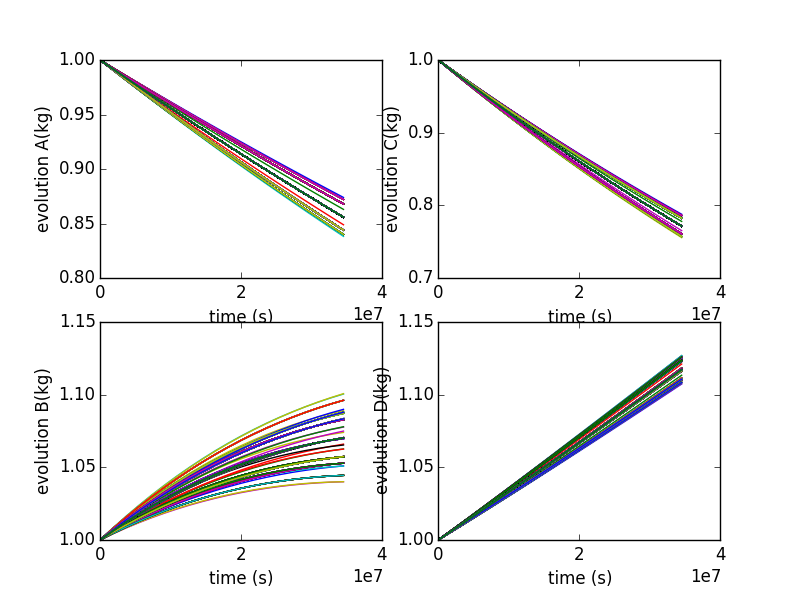
\includegraphics[scale=0.7]{pics/histories_SparseGrid.png}
  \caption{Plot of the samples generated by the Stratified sampling for variables $A,B,C,D$.}
  \label{fig:historiesSparseGridPlotLine}
 \end{figure}
 %%%%%%%%%%%%%%%%%%%%%%%%%%%%%%%%%%%%%%%%%%%%%%%%%%%%%%%%%%
 %%%%%%%%%%%%%%%%%%%%%%%%%%%%%%%%%%%%%%%%%%%%%%%%%%%%%%%%%%
   \item \textbf{\textit{Steps}}:
\begin{lstlisting}[style=XML,morekeywords={arg,extension,pauseAtEnd,overwrite}]
  <Steps>
    <MultiRun name="sample">
      <Input class="Files" type="input">referenceInput.xml</Input>
      <Model class="Models" type="Code">testModel</Model>
      <Sampler class="Samplers" type="SparseGridCollocation">NSG</Sampler>
      <Output class="DataObjects" type="PointSet">samples</Output>
      <Output class="DataObjects" type="HistorySet">histories</Output>
    </MultiRun>
    <RomTrainer name="Ntrain">
        <Input class="DataObjects" type="PointSet">samples</Input>
        <Output class="Models" type="ROM">NROM</Output>
    </RomTrainer>
    <MultiRun name="sampleROM" pauseAtEnd="false">
        <Input class="DataObjects" type="PointSet">inputPlaceHolder</Input>
        <Model class="Models" type="ROM">NROM</Model>
        <Sampler class="Samplers" type="SparseGridCollocation">NSG</Sampler>
        <Output class="DataObjects" type="PointSet">samplesROM</Output>
    </MultiRun>
    <IOStep name="writeHistories" pauseAtEnd="True">
        <Input class="DataObjects" type="HistorySet">histories</Input>
        <Input class="DataObjects" type="PointSet">samples</Input>
        <Input class="DataObjects" type="PointSet">samplesROM</Input>
        <Output 	class="OutStreams" type="Plot">samplesPlot3D</Output>
        <Output 	class="OutStreams" type="Plot">historyPlot</Output>
        <Output 	class="OutStreams" type="Plot">samplesROMPlot3D</Output>
        <Output 	class="OutStreams" type="Print">samples</Output>
        <Output 	class="OutStreams" type="Print">samplesROM</Output>
        <Output 	class="OutStreams" type="Print">histories</Output>
    </IOStep>
  </Steps>
\end{lstlisting}
  %%%%%%%%%%%%%%%%%%%%%%%%%%%%%%%%%%%%%%%%%%%%%%%%%%%%%%%%%%
 %figure samples
 \begin{figure}[h!]
  \centering
  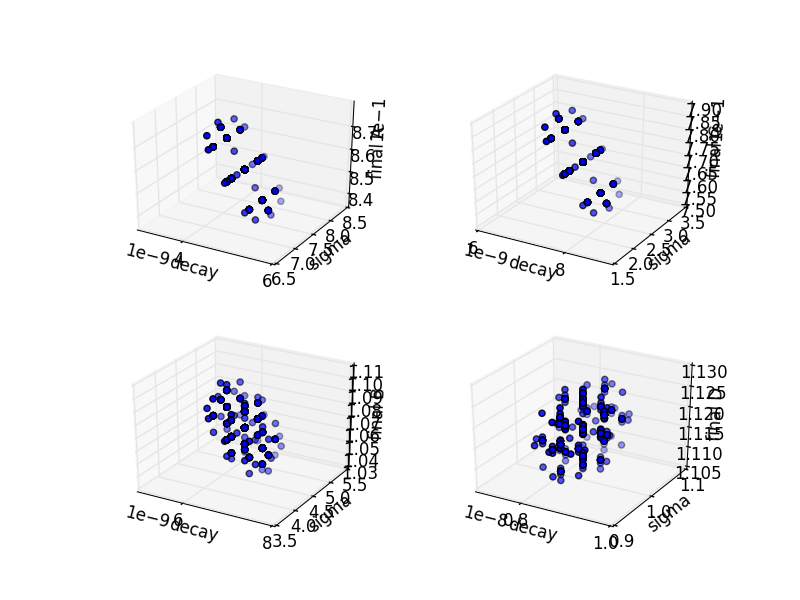
\includegraphics[scale=0.7]{pics/samples_SparseGrid.png}
  \caption{Plot of the samples generated by the Stratified sampling for variables $A,B,C,D$.}
  \label{fig:samplesSparseGridPlotLine}
 \end{figure}
 %%%%%%%%%%%%%%%%%%%%%%%%%%%%%%%%%%%%%%%%%%%%%%%%%%%%%%%%%%
   Finally, the previously defined \textbf{Entities} can be combined in
   the \xmlNode{Steps} block. As inferable,
   four \xmlNode{Steps} have been inputted:
   \begin{itemize}
     \item \xmlNode{MultiRun} named ``sample'', used to run the multiple
     instances of the driven code and
     collect the outputs in the two \textit{DataObjects}. As it can be
     seen, the \xmlNode{Sampler} is inputted to communicate to the
     \textit{Step} that the driven code needs to
     be perturbed through the Sparse Grid Collocation  sampling;
     \item \xmlNode{RomTrainer} named ``Ntrain'', used to train (i.e.,
     construct) the GaussPolynomial ROM. This step is essential if the
     user want to use the ROM in later steps;
     \item \xmlNode{MultiRun} named ``sampleROM'', used to run the multiple
     instances of the previously constructed ROM and
     collect the outputs in the \textit{samplesROM} \textit{DataObjects}.
     As it can be seen, the same Sparse Grid Collocation sampler is
     here used.
     \item  \xmlNode{IOStep} named ``writeHistories'', used to 1) dump
     the ``histories'', ``samples'' and ``samplesROM'' \textit{DataObjects}
     \textbf{Entity} in a CSV file and 2) plot the data in the PNG file and
     on the screen.
   \end{itemize}
\end{enumerate}
 As previously mentioned, Figure~\ref{fig:historiesSparseGridPlotLine}
 shows the evolution of the outputs $A,B,C,D$ under uncertainties.
 Figures~\ref{fig:samplesSparseGridPlotLine} and
 \ref{fig:samplesROMSparseGridPlotLine} show the final responses
 of the sampling employed using the driven code and the ROM,
 respectively. As it can be seen, the constructed ROM can perfectly
 represent the response of the driven code. This example shows the
 potential of reduced order modeling, in general, and of the
 \textit{GaussPolynomialRom}, in particular.

  %%%%%%%%%%%%%%%%%%%%%%%%%%%%%%%%%%%%%%%%%%%%%%%%%%%%%%%%%%
 %figure samples
 \begin{figure}[h!]
  \centering
  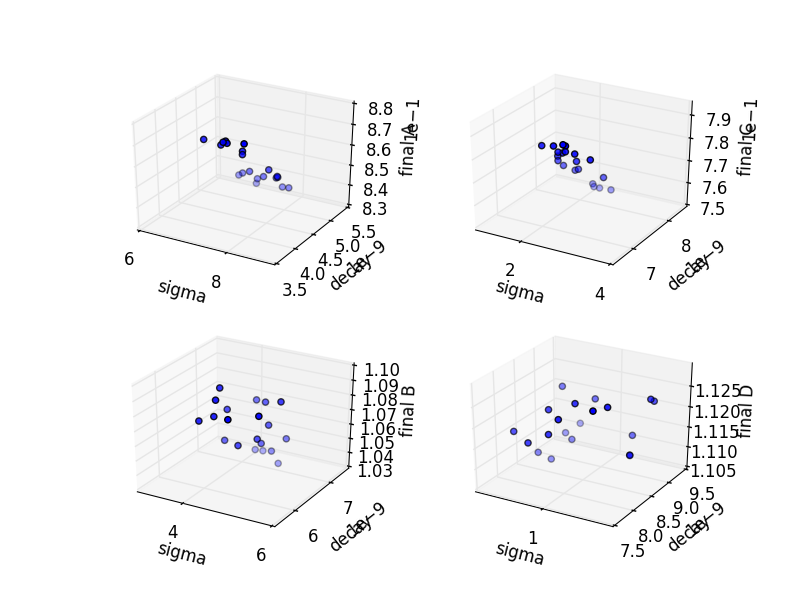
\includegraphics[scale=0.7]{pics/samplesROM_SparseGrid.png}
  \caption{Plot of the samples generated by the Stratified sampling for variables $A,B,C,D$.}
  \label{fig:samplesROMSparseGridPlotLine}
 \end{figure}
 %%%%%%%%%%%%%%%%%%%%%%%%%%%%%%%%%%%%%%%%%%%%%%%%%%%%%%%%%%








